% Figure list
% 1) fig:Coverage
% 2) fig:BGPSMontage
% 3) fig:Bandpass
% 4) fig:Array
% 5) fig:CalibrationCurves
% 6) fig:Flatfield
% 7) fig:CygnusComparison
% 8) fig:PointingCalibrators
% 9) fig:PointingModel
% 10) fig:SCUBAPointingComparison
% 11) fig:IterativeMapping
% 12) fig:Flagging
% 13) fig:GlitchDistribution
% 14) fig:PCA_Graphical
% 15) fig:Deconvolution
% 16) fig:Noise
% 17) fig:NoiseVsLongitude
% 18) fig:PCA_Filter
% 19) fig:AperturePhotometry

% Major Sections
% sec:Introduction
% sec:Observations
% sec:FluxCalibration
% sec:Astrometry
% sec:Mapping
% sec:Noise
% sec:Photometry
% sec:FinalMaps
% sec:Discussion

% calibration
% you should look @ calibration/plot_dcfluxes.pro in my publish/ directory, and /usb/scratch1/planets/planet_dcfluxes.txt is the actual raw data
%/home/milkyway/student/ginsbura/bgps_pipeline/calibration/plot_dcfluxes.pro?

% glitches
% I can't send you raw data for the glitches, but the best way I can think of dealing with them is taking one of my postiter.sav files in some directory and grabbing ac_bolos[where(flags)]...... except that include hand-flagged stuff too

%%%%%%%%%%%%%%%%%%%%%%%%%%%%%%%%%%%%%%%%%%%%%%%%%%%%%%%%%
%                                                       % 
%       Bolocam Galactic Plane Survey Description       %
%                                                       % 
%%%%%%%%%%%%%%%%%%%%%%%%%%%%%%%%%%%%%%%%%%%%%%%%%%%%%%%%%

\documentclass[12pt,preprint]{aastex}
%{emulateapj}

\usepackage{rotating}
\usepackage{subfigure}
\usepackage{datetime}
\usepackage{fmtcount}

\newtimeformat{edttime}{\twodigit{\THEHOUR}:\twodigit{\THEMINUTE}~EDT}
\settimeformat{edttime}
\newdateformat{eurodate}{\dayofweekname{\THEDAY}{\THEMONTH}{\THEYEAR} \THEDAY \monthname[\THEMONTH] \THEYEAR}


\citestyle{aa}

\bibliographystyle{apj_w_etal}

\newcommand{\vect}[1]{\mathbf{#1}}
\newcommand{\xad}{\vect{x}}

\newcommand{\vdag}{(v)^\dagger}
\newcommand{\myemail}{{\tt jaguirre@sas.upenn.edu}}
\newcommand{\lsim}{{_{<}\atop^{\sim}}}
\newcommand{\gsim}{{_{>}\atop^{\sim}}}
\newcommand{\etal}{{et al.\/}}
\newcommand{\ie}{{\em ie.\/}}
\newcommand{\cmq}{cm{$^{-3}$}}
\newcommand{\per}{$^{\rm{-1}}$}
\newcommand{\tc}{{$\theta^1$~Orionis~C}}
%\newcommand{\msol}{M{$_{\odot}$}}
\def\msol{\ifmmode {\>M_\odot}\else {$M_\odot$}\fi}
\newcommand{\lsol}{L{$_{\odot}$}}
\newcommand{\kms}{km~s{$^{-1}$}}
\newcommand{\hii}{H~{\sc ii}}
\newcommand{\Hii}{H~{\sc ii}}
\newcommand{\Ha}{\mbox{H$\alpha$}}
\newcommand{\sii}{S~{\sc ii}}
\newcommand{\Feii}{Fe~{\sc ii}}
\newcommand{\oi}{O~{\sc i}}
\newcommand{\nii}{N~{\sc ii}}
\newcommand{\oiii}{O~{\sc iii}}
\newcommand{\mgii}{Mg~{\sc ii}}
\newcommand{\tco}{{$^{13}$CO}}
\newcommand{\CO}{{$^{12}$CO}}
\newcommand{\Tco}{{$^{12}$CO}}
\newcommand{\co}{C{$^{18}$O}}
\newcommand{\Lsol}{L$_{\odot}$}
\newcommand{\Msol}{M$_{\odot}$}
%\newcommand{\C18o}{C$^{18}$O($1\rightarrow 0$)}
\newcommand{\Check}{{\bf ???}}
\newcommand{\mum}{\ensuremath{\mu \mathrm{m}}}
\newcommand{\flux}{flux density}
\newcommand{\solar}{\ensuremath{\odot}}

\newcommand{\epsi}{\varepsilon}

% -----------------------------------------------------------------------------
% BGPS specific definitions
\def\bgps{BGPS}
\newcommand{\bgpsarea}{150}
\newcommand{\bcamfwhm}{31.2\arcsec}
\newcommand{\ncores}{7628}
\newcommand{\bgpsdepthlow}{20}
\newcommand{\bgpsdepthhigh}{50}
% -----------------------------------------------------------------------------

\newcommand{\TBD}{{\bf TBD}}

\def\Figure#1#2#3#4{
\begin{figure}[htb]
\epsscale{#4}
\plotone{#1}
\caption{#2}
\label{#3}
\end{figure}
}

\def\FigureTwo#1#2#3#4#5{
\begin{figure}[htb]
\epsscale{#5}
\plottwo{#1}{#2}
\caption{#3}
\label{#4}
\end{figure}
}


\def\Table#1#2#3#4#5{
\begin{deluxetable}{#1}
\tablewidth{0pt}
\tablecaption{#2}
\tablehead{#3}
\startdata
\label{#4}
#5
\enddata
\end{deluxetable}
}

\newcommand{\penn}{1}
\newcommand{\casa}{2}
\newcommand{\utexas}{3}
\newcommand{\virginia}{4}
\newcommand{\ucf}{5}
\newcommand{\wisc}{6}
\newcommand{\jpl}{7}
\newcommand{\ubc}{8}
\newcommand{\hawaiihilo}{9}
\newcommand{\hawaiimain}{10}
\newcommand{\arizona}{11}

	% End definitions

\slugcomment{DRAFT: \currenttime\ \eurodate\today}

\shorttitle{BGPS}
\shortauthors{Aguirre et al.}

\begin{document}

\title{The Bolocam Galactic Plane Survey: Survey Description and Data
Reduction}

%\newpage
%\pagebreak
%
%\tableofcontents
%
%\newpage
%\pagebreak
%


\author{James Aguirre\altaffilmark{\penn},
        Adam Ginsburg\altaffilmark{\casa},
        Miranda Nordhaus\altaffilmark{\utexas},
	Meredith Drosback\altaffilmark{\virginia},
        John Bally\altaffilmark{\casa}, 
	Cara Battersby\altaffilmark{\casa},
	Eric Todd Bradley\altaffilmark{\ucf},
%        Richard Chamberlin\altaffilmark{\cso},
	Claudia Cyganowski\altaffilmark{\wisc},
	Darren Dowell\altaffilmark{\jpl}
	Neal J. Evans II\altaffilmark{\utexas},
        Jason Glenn\altaffilmark{\casa},
        Paul Harvey\altaffilmark{\utexas,\casa},
        Erik Rosolowsky\altaffilmark{\ubc},
%        Wayne Schlingman\altaffilmark{9},
%        Yancy Shirley\altaffilmark{9},
        Guy S. Stringfellow\altaffilmark{\casa},
        Josh Walawender\altaffilmark{\hawaiihilo}, and 
        Jonathan Williams\altaffilmark{\hawaiimain}
}

\affil{{$^\penn$}{\it{Department of Physics and Astronomy, University of
      Pennsylvania, Philadelphia, PA }}}
\email{\myemail}

\affil{{$^\casa$}{\it{CASA, University of Colorado, CB 389, Boulder, CO 80309}}}
%, \email{John.Bally@casa.colorado.edu}
%      \email{adam.ginsburg@colorado.edu}
%      \email{cara.battersby@colorado.edu}
%      \email{Jason.Glenn@colorado.edu} \email{pmh@astro.as.utexas.edu}
%      \email{Guy.Stringfellow@colorado.edu} }}


\affil{{$^\utexas$}{\it{Department of Astronomy, University of Texas,
      1 University Station C1400, Austin, TX 78712}}}
%,            
%      \email{nje@astro.utexas.edu},
%      \email{nordhaus@astro.utexas.edu}}}

\affil{{$^\virginia$}{\it{Department of Astronomy, University of
Virginia, P.O. Box 400325, Charlottesville, VA 22904}}}
%, 
%    \email{meredith.drosback@origins.colorado.edu}}}

\affil{{$^\ucf$}{\it{Department of Physics, University of Central
Florida}}}
%,           
%                                              } ,   \email{tbradley@physics.ucf.edu}} }  

\affil{{$^\wisc$}{\it{Department of Astronomy, University of Wisconsin,
       Madison, WI 53706}}}
% , \email{cyganow@astro.wisc.edu}}}

\affil{{$^\jpl$}{\it{Jet Propulsion Laboratory, California Institute
   of Technology, 4800 Oak Grove Dr., Pasadena, CA 91104}}}
%,
%       \email{cdd@submm.caltech.edu}}}

\affil{{$^{\ubc}$}{\it{Department of Physics and Astronomy, University
       of British Columbia, Okanagan }}}
% ,               \email{erik.rosolowsky@ubc.ca}}} 

%\affil{{$^{\arizona}$}{\it{ Steward Observatory, University of
%Arizona, 933 North Cherry Avenue, Tucson, AZ 85721 }}}
%%\email{yshirley@as.arizona.edu} \email{wschlingman@as.arizona.edu}}}

\affil{{$^{\hawaiihilo}$}{\it{Institute for Astronomy, University of
        Hawaii,640 N. Aohoku Pl., Hilo, HI 96720}}}
%\email{joshw@ifa.hawaii.edu} }}

\affil{{$^{\hawaiimain}$}{\it{Institute for Astronomy, University of
Hawaii,680 Woodlawn Drive, Honolulu, HI 96822}}}
%\email{jpw@ifa.hawaii.edu}}

%\altaffiltext{\penn}{University of Pennsylvania, Philadelphia, PA 19104}
%%Jansky Fellow, National Radio Astronomy Observatory} 
%\altaffiltext{\casa}{CASA, University of Colorado, CB 389, Boulder, CO 80309}
%\altaffiltext{\utexas}{Department of Astronomy, University of Texas, 
%       1 University Station C1400, Austin, TX 78712}
%\altaffiltext{4}{Caltech Submillimeter Observatory, Hilo, HI}
%\altaffiltext{5}{Institute for Astronomy (IfA), University of Hawaii
%640 N. Aohoku Pl., Hilo, HI 96720}
%
\begin{abstract}

We present the Bolocam Galactic Plane Survey (BGPS), a 1.1 mm
continuum survey of \bgpsarea\ square degrees of the Galactic Plane in
the 1st, 2nd, and 3rd quadrants.  The BGPS represents the first large
area, systematic survey of the Northern Galactic Plane in the
(sub)millimeter continuum without pre-selected targets.  The survey
has detected \ncores\ clumps to a limiting depth of between
\bgpsdepthlow\ and \bgpsdepthhigh\ mJy RMS.  We include maps of 100
contiguous square degrees from $l=-10.5$ to $l=86.5$ and $b=\pm0.5$
with a resolution of 31\arcsec, as well as regions in IC1396, $l=111$
(NGC7538), W3/4/5, and Gem OB1.  The most striking feature of the maps
is the filamentary structure of cold dust throughout the Galaxy.

This paper details the survey observations and methods.  We treat
carefully the determination of pointing and flux calibration errors
and compare our results to the literature.  Data processing algorithms
that separate astronomical signals from time-variable atmospheric flux
in the data time-stream are discussed.  The algorithms reproduce the
structure of the astronomical sky on a limited range of angular scales
and produce artifacts in the vicinity of bright sources. Specifically,
extended emission smooth on scales larger than about 5\arcmin\ is not
fully recovered in the images.  The spatial frequency response
function of the Bolocam Galactic Plane Survey is discussed.

This paper serves as a companion and guide to the public data release
through NASA's Infrared Processing and Analysis Center (IPAC).  These
images represent an important finder chart for future observations
with ALMA and a long-wavelength spectral band complementary to
imminent submillimeter surveys with SCUBA-2 and Herschel-SPIRE.

\end{abstract}

\keywords{
ISM: - molecular clouds --
stars: formation -- high mass
millimeter continuum
}

%\include{bgps_methods_introduction}

\section{Introduction}
\label{sec:Introduction}

Millimeter-wavelength continuum surveys of the Galactic plane provide
the best way to identify high-column density clumps and clumps where
planets, stars, and star clusters form.  Such data can locate and lead
to the measurement of the physical properties of clumps un-biased by
selection effects such as the presence of embedded stars, star
clusters, infrared sources, masers, or radio continuum emission.
Galaxy-wide surveys are essential for measuring the impacts of the
environment on clump properties and star formation activity.  Do clump
properties vary with location in or out of spiral arms?  Do clump
properties vary with Galactocentric distance?  Do they depend on the
level of nearby star formation activity?  Galactic plane surveys of
mm-wavelength dust continuum emission provide the most efficient tool
for the identification of potential or active sites of star formation,
including the rare objects where the most massive stars and cluster
are, or soon will be, forming.  Dust continuum surveys of the Galaxy
provide essential ``ground truth'' required for the analysis of distant
galaxies where where individual clouds and clumps are not resolved and
only galaxy-wide average quantities can be measured.

Dust continuum emission near a wavelength of 1 mm is the best tracer
of the material most directly associated with the formation of
planetary systems, stars, and star clusters \citep{johnstone06}.
Galactic dust continuum radiation at this wavelength is optically-thin
almost everywhere, and at typical dust temperatures of order 10 K or
more, is observed on the Rayleigh-Jeans tail of the Planck function.
Thus, the determination of column densities is relatively straight
forward if the dust temperature is known.

Submillimeter observations of Galactic sources have been conducted by
a variety of different groups focusing on small regions since
bolometer technology was developed.  The Submillimeter Common-User
Bolometer Array (SCUBA) on the 15 m James Clerk Maxwell Telescope
mapped many significant regions in the galactic plane over its 8 year
lifetime \citep{holland99,difrancesco08}, but never completed a
contiguous survey of the galactic plane.  Bolocam and Mambo have
previously been used to map large star forming regions at 1.1
\citep{enoch06} and 1.2 mm \citep{motte07}, but again these were
targeted observations.  A recent large area survey with the LABOCA
instrument at 870 \mum\ has recently been reported \citep{schuller09}.

Surveys of the galaxy in CO line emission \citep{dame01,FCRAO} have
revealed much about galactic structure, but do not provide a complete
picture of how star formation follows that structure.  Millimeter
continuum more directly traces the cold dust associated with star
formation.  Continuum data allows for accurate determinations of the
mass of large, dense dust structures when combined with kinematic
distances \citep[e.g.][]{RotationCurve}.

A crucial step in the observational study of star and cluster
formation is identification and characterization of the cloud clumps
which will soon form or are actively forming stars.  Massive stars and
clusters form from high-density cloud clumps with very large column
densities and extinctions $A_V > $ 100.  Thus, such cloud clumps are
best investigated at millimeter and sub-millimeter wavelengths.
However, the interpretation of various gas tracers that produce
emission lines in this portion of the spectrum is very difficult.
Although in principle, spectral lines provide excellent diagnostics of
line-of-sight motions, temperatures, and densities in a cloud,
variations in tracer abundances caused by depletions and complex
chemical processing, uncertainties in excitation conditions, and the
impacts of radiation fields and shocks make the derivation of column
densities, masses, and other physical properties of cloud clumps very
difficult.  The continuum emission from warm dust provides a more
reliable tracer of the column densities and clump masses.

The advent of focal plane arrays containing hundreds of individual
bolometers sensitive to millimeter and sub-millimeter (sub-mm)
radiation has enabled large-scale surveys of mm-wavelength continuum
emission from Galactic interstellar dust.  The great advantage of
continuum observations at 1.1mm is the low optical depth of the dust,
permitting an estimate of the mass of the emitting region.  Further,
the mass column density is independent of the gas volume density.

Using the same dust opacity as \TBD\ ({\it put in original references})
%\citet{enoch06} and \citet{young06},
and assuming a gas-to-dust mass ratio $X$ of 100, the mass sensitivity
can be written as
\begin{equation} 
\label{eq:Mass}
M_{gas}\approx
0.22\left( e^{12.9/T_d}-1 \right) \left({S_\nu\over 15\; {\rm mJy}} \right)
D^{2}_{kpc} \msol 
\end{equation}
where $D_{kpc}$ is the distance to the source in kpc.  (At $S_\nu =
15$~mJy this corresponds to an RMS extinction sensitivity of $A_V\sim
1$ mag, with the same $T_d$ dependence).  For Bolocam, $h\nu/k \approx
13$~K, so for $T_d > XXX$ the dependence is approximately linear.  At
the coldest temperatures expected, the mass changes a factor of 2.9
between 20 and 10 K.  Far more important is the accurate determination
of the distance to the clump.

Thus it is thus possible with a wide area, relatively shallow 1.1~mm
survey to provide an unmatched, uniform inventory of massive
star-forming and starless condensations.

This survey presents the results of one of the first wide-area,
untargeted surveys of the Galactic Plane in the millimeter continuum.
We have used the 144 element Bolocam focal plane array, mounted at the
Cassegrain focus of the 10 meter diameter sub-mm telescope at the
Caltech Sub-millimeter Observatory (CSO), to survey over \bgpsarea\
square degrees of the northern Galactic plane at a wavelength of 1.1
mm in the dust continuum.  Figure \ref{fig:Coverage} shows the
coverage of the \bgps.  Maps of the entire BGPS are presented in
Figure \ref{fig:BGPSMontage}.  We have detected \ncores\ clumps in the
surveyed fields, providing an unbiased sample of clumps suitable for
multi-wavelength and high-resolution studies with existing telescopes
and future facilities.  The clump catalog is described in a companion
paper \citep{rosolowsky09}.

At the distances that we are observing these objects, we are likely
observing aggregates of star forming cores found in a larger molecular
cloud environment, which we will refer to as clumps
\citep{williams00}.


The outline of the paper is as follows. Section \ref{sec:Observations}
describes the instrument and the observations.  Section
\ref{sec:FluxCalibration} describes the flux calibration and errors.
Section \ref{sec:Astrometry} describes the construction of an absolute
reference frame for the observations and verification against other
(sub)millimeter catalogs.  Section \ref{sec:Mapping}, \ref{sec:Noise},
\ref{sec:Photometry}, \ref{sec:FinalMaps}, \ref{sec:Discussion}.

%BGPS will identify regions of high-mass star and cluster formation
%throughout the Galaxy and sites of low-mass star formation within a
%few kpc of the Sun (Figure 1).  Their physical properties may then be
%constrained by comparison with data in other wavebands.  The
%distribution of these regions will be compared with other tracers of
%the interstellar medium (ISM) such as molecular clouds, supershells,
%HII regions, supernova remnants, and supershells.  The 1.1 mm data
%together with dust continuum maps at shorter wavelengths taken by us
%with SHARC~II or with other telescopes will constrain temperature and
%reveal what surrounding material may be feeding the formation of dense
%cores. Star formation efficiencies may be obtained by detailed
%comparison of the NIR-MIR observations of stars with the BGPS
%observations.  This will also constrain the extinction law and dust
%properties, essential to refining mass estimates.  By comparing the
%distribution of 1.1mm cores with HII regions, supernova remnants, and
%IR emission as seen by {\it Spitzer}, we will constrain the mode of
%core and star formation, i.e., is it predominantly triggered by
%advancing shock and ionization fronts, by converging flows in a
%turbulent medium, or by spontaneous gravitational collapse?  The
%former models predict a close correlation between fronts and cores
%while the latter predicts the correlation will be poor.


%\Figure{mass_limits}{The limiting gas mass of cores detectable
%with at a flux limit of 15 mJy RMS. Detection thresholds at 3 (dashed)
%and 5 (solid) $\sigma$ are shown for a range of dust temperatures.
%Dust temperatures $<20$~K are most interesting for this survey, since
%these are the sources most likely to be pre- or proto-stellar
%condensations.}{fig:mass_limits}{1.0}
%
\Figure{coverage_moll} {The coverage of the BGPS.  The background
greyscale is IRAS 100 \mum.  
%The Bolocam coverage is shown with white
%solid lines in the top two panels and black in the bottom three.
%Major regions of Galactic star formation are labeled.  The coverage of
%{\em Spitzer}-GLIMPSE \citep{benjamin03} and the FCRAO $^{13}$CO GRS
%\citep{jackson06} are shown.
}{fig:Coverage}{1.0}

% TEST
% Useful, but not here
%\begin{figure}
%  \subfigure[$l=-10.5$ to $l=19.5$ Units are Jy/Beam.  The brightest
%	sources, e.g. Sgr B2, Sgr A, and sources near $l=10$ and
%	$l=13$, appear to be saturated, but this is only a display
%	artifact.  The noise is more pronounced from $l=-7$ to $l=-2$
%	because this region was observed less.]{\label{fig:BGPSMontage-a}\includegraphics[scale=0.75]{fig1_pg1_bw_inv_bar_label}}\\
%\pagebreak
%\subfigure[$l=19.5$ to $l=49.5$.  Units are Jy/Beam .  G34.3+0.15, W
%	51, W 43, W 49, and M 17 appear to be saturated, but this is
%	only a display artifact.]
%{\label{fig:BGPSMontage-b}\includegraphics[scale=0.75]{fig1_pg2_bw_inv_bar_label}}
%
%\end{figure}
%% --------------------------------
%


\newcounter{subfig}
\setcounter{subfig}{1}
\renewcommand{\thefigure}{\arabic{figure}\alph{subfig}}

%\begin{sidewaysfigure}[h]
\begin{figure}
  \begin{minipage}{6.5in}
    \begin{center}
 %     \includegraphics[scale=0.9]{fig1_pg1_bw_inv_bar_label}
      \caption{$l=-10.5$ to $l=19.5$ Units are Jy/Beam.  The brightest
	sources, e.g. Sgr B2, Sgr A, and sources near $l=10$ and
	$l=13$, appear to be saturated, but this is only a display
	artifact.  The noise is more pronounced from $l=-7$ to $l=-2$
	because this region was observed less.}
    \end{center}
    \label{fig:BGPSMontage}
  \end{minipage}
\end{figure}
  
\addtocounter{figure}{-1}
\addtocounter{subfig}{1}

\begin{figure}
  \begin{minipage}{6.5in} 
    \begin{center}
 %     \includegraphics[scale=0.9]{fig1_pg2_bw_inv_bar_label} 
      \caption{$l=19.5$ to $l=49.5$.  Units are Jy/Beam .  G34.3+0.15, W
	51, W 43, W 49, and M 17 appear to be saturated, but this is
	only a display artifact}
    \end{center}
  \end{minipage}
\end{figure}

\addtocounter{figure}{-1}
\addtocounter{subfig}{1}

\begin{figure}
  \begin{minipage}{6.5in} 
    \begin{center}
%      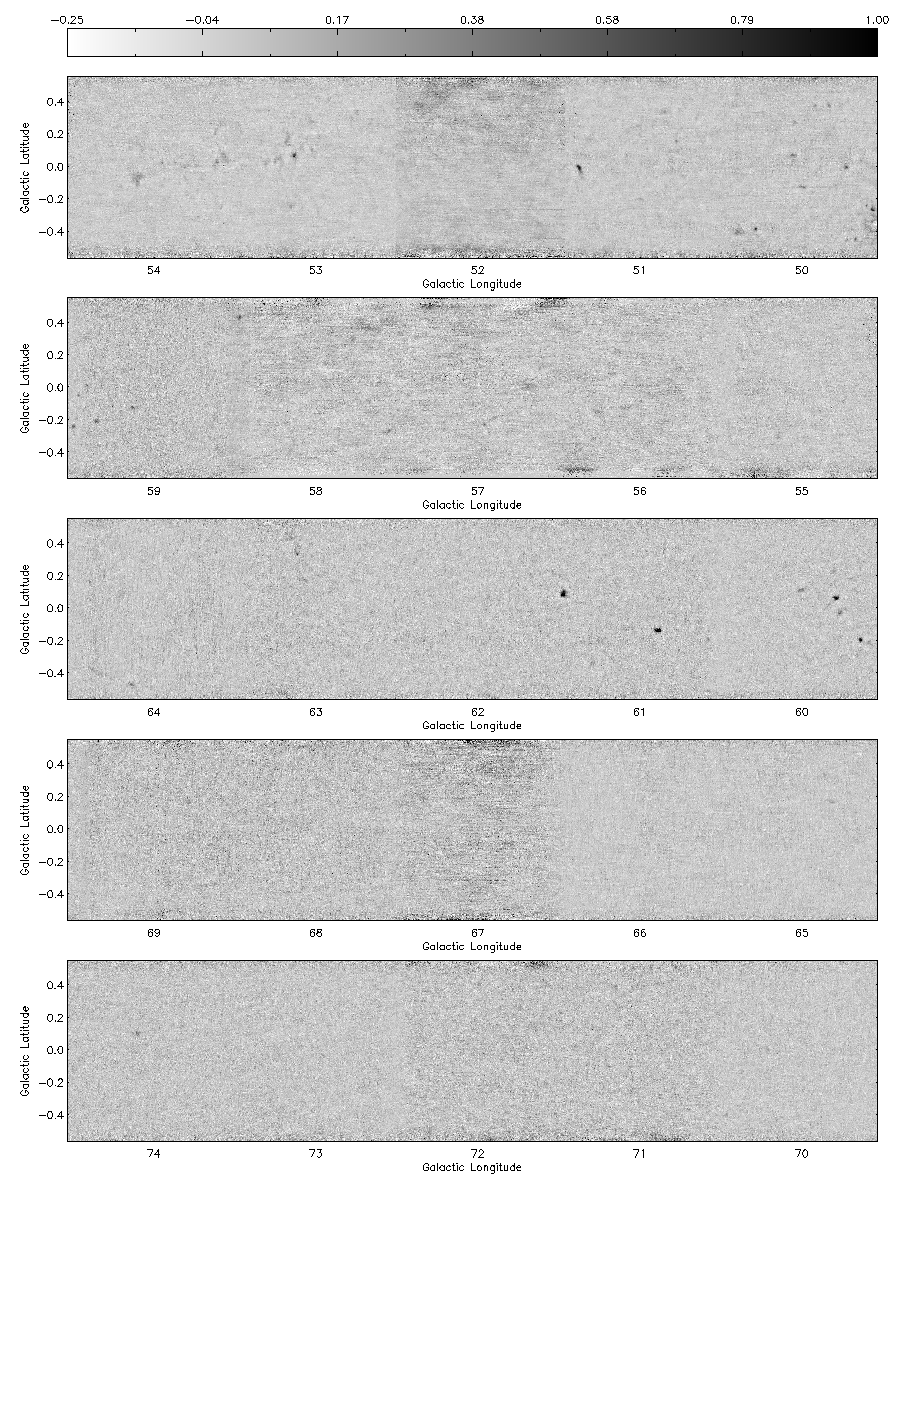
\includegraphics[scale=0.9]{fig1_pg3_bw_inv_bar_label}
      \caption{$l=49.5$ to $l=74.5$.  \TBD\ Add annotations}
    \end{center}
  \end{minipage}
\end{figure}

\addtocounter{figure}{-1}
\addtocounter{subfig}{1}

\begin{figure}
  \hspace{-1in}
%  \includegraphics[scale=0.8]{fig1_pg5_bw_inv_bar_label} 
  \caption{The Cygnus Arm. \TBD\ Add annotations}
\end{figure}
%  \vspace{-4in}

\addtocounter{figure}{-1}
\addtocounter{subfig}{1}

\begin{figure}
\hspace{-0.5in}
%  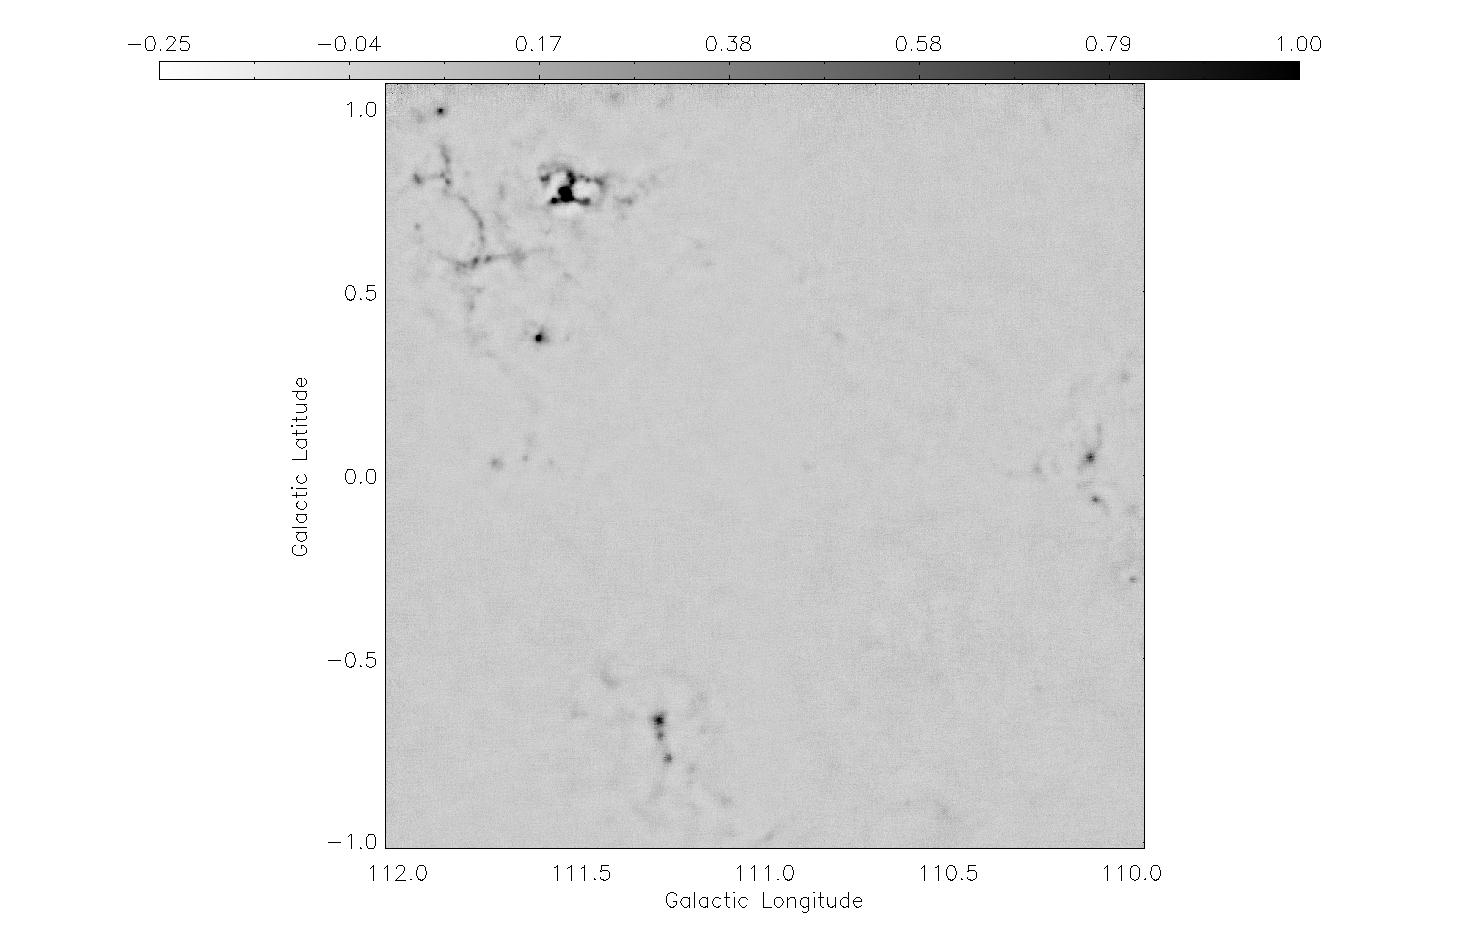
\includegraphics[scale=0.8]{fig1_pg4_bw_inv_bar_label} 
  \caption{Cloud complexes centered at $l=111$ in the Perseus Arm. \TBD\ Add annotations}
\end{figure}

\addtocounter{figure}{-1}
\addtocounter{subfig}{1}

\begin{figure}
  \hspace{-1in}
%  \includegraphics[scale=0.8]{fig1_pg6_bw_inv_bar_label} 
  \caption{W3/4/5 \TBD\ Add annotations}
\end{figure}

\renewcommand{\thefigure}{\arabic{figure}}

\clearpage

%\include{bgps_methods_observations}
\section{Observations}
\label{sec:Observations}

%\subsection{Instrument}

Bolocam\footnote{{\tt http://www.cso.caltech.edu/bolocam}} is the
facility 144-element bolometer array camera operating from the 10.4 m
dish of the Caltech Submillimeter Observatory (CSO) on the summit of
Mauna Kea.  We used the filter configuration with a bandcenter of
268~GHz (hereafter 1.1~mm) and fractional bandwidth $\Delta \nu/\nu =
0.17$.  The passband is constructed to exclude the $^{12}\mathrm{CO}(2
\to 1)$ emission line.  Figure \ref{fig:Bandpass} shows the passband.
We compute color corrections for sources of varying spectral index in
Appendix \ref{app:ColorCorrections}.

The array field-of-view is 7\arcmin.5, with individual detectors
having nearly Gaussian beams of \bcamfwhm\ FWHM.  The spacing of the
pixels at 1.1 mm is 1.6$f\lambda$, so the focal plane is not
instantaneously sampled.  The Bolocam instrument is described in greater
detail in \citet{haig04} and \citet{glenn03}.

%\subsection{Observations}

The observations described here were acquired during six separate
observing sessions at the CSO over the course of two years.  The
observing epochs are given in Table \ref{tab:Observing}, along with
corresponding ranges for the zenith opacity $\tau_{225}$ of the CSO
tipper tau.  Because of the CSO weather multiplexing policy, Bolocam
observations were typically scheduled when $\tau_{225} > 0.06$.
Between each observing epoch, Bolocam was removed from its mount at
the re-imaged Cassegrain focus and stored warm.  Thus the flux
calibration and pointing model must be re-computed for each epoch to
allow for variations in the instrument and optics.  We found that the
flux calibration did not in fact differ significantly between epochs.
For the pointing model, we computed a well-constrained version for
Epoch V and aligned all images to this.

%\subsection{Observing Strategy}

% xraster 120 11280 23 /step_size=162 /equatorial /position_angle=36.753118 /alternate_direction /rot /settling_time = 03

Our basic observing strategy was to raster scan Bolocam by moving the
primary mirror of the CSO to modulate the astrophysical signal faster
than fluctuations in atmospheric opacity.  Each field was scanned with
alternating raster scans along $l$ and $b$.  Starting with Epoch III,
the fundamental scan unit was a $3\arcdeg \times 1\arcdeg$ block.
Each block was scanned with 23 scans along lines of constant $b$, and
67 scans along lines of constant $l$.  In both cases, the spacing
between adjacent rasters was 162\arcsec.  The total time for such a
scan was between 39 and 48 minutes.  The data were electronically
sampled at 10 Hz along the scan direction, slightly higher than the
Nyquist rate for the scan speed of 120\arcsec\ s$^{-1}$.


In order to fill in the instanteously undersampled focal plane, we
began using in Epoch II a field rotator to mechanically align the
focal plane at an optimal orientation along the scan direction to
improve the sampling orthogonal to the scan direction.  This is shown
in Figure \ref{fig:Array}.  Achieving good sampling is complicated by
a number of missing pixels.  A simulation was performed to determine
the optimal angle to rotate the array with respect to the scan
direction to account for the beam spacing and missing pixels.  During
the turnaround following a raster, the field rotator is adjusted to
this optimum angle.
%CHECK
% per Adam, 2009/3/26
Without the field rotator, the coverage shows variations of 100\% from
pixel to pixel in a single raster of a field.  With the rotator, this
is reduced to $\sim40\%$.  

% FIGURES AND TABLES

\Figure{bolocam_bandpass}{The Bolocam 1.1 mm bandpass.  Bright
molecular emission lines are shown at their rest frequencies.  Note
that the Bolocam passband rejects $>90\%$ of the $^{12}$CO flux,
leaving our continuum measurements largely uncontaminated.  SO and
CH$_3$OH lines are probably the dominant contributors to line flux in
the passband.  \citet{nummelin1998} found that 22\% of the flux in one
pointing towards Sgr B2 was from lines, and \citet{yoshida2005}
reported $>40\%$ in Orion A from line emission. \TBD\ Other lines
lying in the Bolocam passband include CS($5\to4$) and ($6\to5$) (245
and 293 GHz), HCN($3\to2$) (265 GHz) and HCO$^+(3\to2)$ (267 GHz).}
{fig:Bandpass}{1.0}

\Table
{lllll}
{Observing Epochs for the BGPS}
{Number & Begin (UT) & End (UT) & Nights & $\tau_{225}$ }
{tab:Observing}
{
I   & 2005 Jul 03 & 2005 Jul 13 & 5 & 0.1 \\
II  & 2005 Sep 04 & 2005 Sep 12 & 5 & 0.1 \\
III & 2006 Jul 01 & 2006 Jul 13 & 5 & 0.1 \\
IV  & 2006 Sep 01 & 2006 Sep 09 & 5 & 0.1 \\
V   & 2007 Jul 01 & 2007 Jul 13 & 5 & 0.1 \\
VI  & 2007 Sep 01 & 2007 Sep 09 & 5 & 0.1 \\
}

\FigureTwo{bolosens050904_o32}{scan_10deg}{Left: the position,
ellipticity and relative response of the detectors in the Bolocam
focal plane as mapped to the sky.  Right: The effect of field rotation
on the coverage obtained via Bolocam raster scans.}{fig:Array}{1.0}

\section{Overview of the Data Reduction}
\label{sec:Overview}

%{\it material from the Letter here}

A number of different descriptions of the reduction of Bolocam data
have been published \citep{laurent05,enoch06,sayers09}.  This work
addresses the issues specific to the BGPS, significantly improving the
method of \citet{enoch06} for generating maps and characterizing their
properties.  It incorporates also some of the technical developments
of \citet{sayers09}, though the exquisite control of systematics and
noise of that analysis is neither necessary nor possible here.

The data were reduced with a custom pipeline written specifically for
the galactic plane survey based on \citet{enoch06} and
\citet{Laurent2006}.  A key element of the reduction is the iterative
estimation of the atmospheric fluctuations and the astrophysical
signal.  The atmospheric model is developed from a set of principal
components of the bolometer signal time series under the assumption
that the bulk of the correlated signal is atmospheric.  The iterative
estimation process then helps to restore correlated flux due to
astrophysical emission \citep[details in][]{Aguirre2009}.

The Bolocam observations are sensitive to structure between 31\arcsec\
and about 400\arcsec\ (the array field of view).  An indicative
analysis of the spatial filter function of the iterative mapping
scheme is given in \citet{enoch06}.  The data were sampled onto a
uniform 7\farcs2 grid.  Flux density calibrations were performed using
observations of Mars, Uranus, and Neptune, and they are accurate to
$\sim$20\%.

%A calibration scheme capable of
%5\% systematic and $<$5\% statistical errors is being implemented as outlined in
%\citet{Sayers2009}.
%To account for offsets between the observations, each observation was mapped
%individually and aligned to a `master' field that has been tied to
%pointing calibrators. 
Noise properties across the survey are not completely uniform, but the
measured $1\sigma$ level is $\approx43\pm7$ mJy/beam within the
$b=\pm.5$ portion of the plane.
%After the pipeline mapping, the fields were combined using the COMBINE
%command in IRAF with WCS offsets.

The absolute pointing accuracy of the survey has been measured to be
$\sim$6\arcsec\ RMS.  A single $3^\circ \times 1^\circ$ observation of
each region was registered to the pointing calibrators as a `master
field,' and additional observations of that field were aligned to the
master.

Bright and large sources leave an impact on their surroundings when
cleaned with a principal component subtraction.  \object{Sgr B2},
\object{G 34.3+0.15}, and other sources with fluxes $\geq 10$ Jy are
surrounded by substantial negative bowls.  Some flux is restored in
these bowls using the iterative process described in
\citet{Aguirre2009}, but around the brightest sources the impact of
the source on the background estimation is too great to be fully
recovered.

Instrument glitches and cosmic ray hits have been removed by a
combination of outlier rejection in each spatial pixel and hand
flagging of the timestream data.  Streaking in the images results from
incorrect determinations of the zero level across scans when a bright
source is encountered.  Atmospheric noise in observations taken in
poor weather may not be completely removed by the reduction
procedures.
%Particular bolometers may be noisy for a single observation and they may not
%be adequately down-weighted. 

\section{Flux Density and Surface Brightness Calibration}
\label{sec:FluxCalibration}

The absolute flux calibration is obtained from observations of Mars
and Uranus
% no good observations, per AG
%and Neptune 
(the ``primary calibrators'').  The millimeter-wave flux of these
planets is known to $\sim 5\%$ \citep{orton86,griffin93}.
Calibrations at (sub)millimeter wavelengths are strongly affected by
atmospheric opacity corrections.  Further, the detector responsivity
of Bolocam's bolometers is a non-linear function of the mean
atmospheric loading.

To relate observations of the primary calibrators to observations of
the BGPS fields, we make use of the following relation.  The
calibration ${\cal S}$, referred to the detectors, is given by
\begin{equation}
\label{eq:Calibration}
{\cal S} \, \left[\mathrm{\frac{V}{Jy}}\right] = 
S(\tau) \eta A \exp{(-\tau)} \Delta\nu
\end{equation}
where $S$ is the bolometer responsivity ([V/W]), $\eta$ is the system
optical efficiency, $A$ is the effective telescope collecting area,
$\Delta \nu$ is the bandwidth, and $\tau$ is the line-of-sight,
in-band atmosphere opacity.  Under the assumption that the only power
variation on the detectors is due to the power from the atmosphere,
which may be parameterized by $\tau$, ${\cal S}$ is a single-valued
function of $\tau$.  We have used the mean bolometer resistance as a
proxy for $\tau$, since the bolometer resistance is a single-valued
function of loading.  {\it This quantity is monitored continuously for
all observations.}  Note that this calibration curve folds in both the
effects of changing atmospheric transmission, as well as changes in
the detector response with optical loading.

%Multiple observations of secondary calibrators suffice to give the
%shape of the curve.  To reference it to the absolute calibrators, the
%fluxes of the planets were held fixed and the fluxes of the secondary
%calibrators allowed to float to produce the best agreement with a
%second-order polynomial for all sources.  The values for the secondary
%calibrators agree well with previously obtained Bolocam values and
%with values in the literature \citep{sandell94,jenness02}.  
%%A fit of Equation \ref{eq:Calibration} 
%

A fit to the observed values for the primary calibrators was performed
for the each epoch separately.
%CHECK
The agreement between epochs was good, so a single combined
calibration was used for all data here.
%We have found that the calibration can differ
%between successive cooldowns of the instrument by $\sim10\%$ \Check\
%but is generally stable over the period of order a month which
%constitutes each of the observing epochs.  
The calibration curve is shown in Figure \ref{fig:CalibrationCurves}.  The
resulting error on the calibration curve fit is less than 
%CHECK
$5\%$ (statistical) over the observed range of $\tau$.  A tally of all
contributions to the flux density error is given in Table
\ref{tab:ErrorBudget}.

The above flux density calibration only accounts for the average
calibration of bolometer Volts to Janskys.  It is also necessary to
account for the variation of bolometer response across the focal
plane.  We do this by monitoring the response to the atmosphere
emission in all bolometers.  Since the atmosphere is common to all
detectors, any changes in response are due to the intrinsic properties
of the detectors.  The change in relative response with loading for a
typical detector is shown in Figure \ref{fig:CalibrationCurves}.  The
actual application of the the method to the time series of the
bolometer data is shown in Figure \ref{fig:Flatfield}, and is
discussed further in Section \ref{sec:Mapping}.

The instrument beam size (PSF) is measured using the planets Uranus
and Neptune which are nearly point sources for Bolocam.
%The semi-diameter of
%Mars over this period ranged from 2.3\arcsec\ to 2.9\arcsec, with
%Neptune $\sim1.1\arcsec$.  Relative to the \bcamfwhm~FWHM Bolocam
%beam, these may be regarded as point sources; the finite size of Mars
%results in a $< 1.5\%$ correction of the observed flux.
The maps of the planets, including all detectors, are fit to a
Gaussian profile.  The beam area is that averaged over all detectors,
and is ?$1.71\times10^{-6}$\TBD\ ($35.6$\farcs) steradians.  This
allows conversion of the maps, calibrated in Jy beam$^{-1}$, into
surface brightness (MJy sr$^{-1}$).  The uncertainty in the beam size
is ?$.7\%$\TBD\ (number quoted is the uncertainty in the mean beam
size), leading to an uncertainty in the surface brightness calibration
of \TBD.

\subsection{Comparison to Other Surveys}

Comparison of the accuracy of the Bolocam flux density calibration
with the SCUBA 850 \mum\ results is complicated by the unknown effect
of the dust spectral index.  However, there are several large-area
surveys with the MAMBO instrument at 1.2 mm with which we can compare.
Figure \ref{fig:CygnusComparison} shows the comparison of fluxes
extracted from our map in the Cygnus Arm with those of
\citet{motte07} (M07).

The figures of the Cygnus-X region presented by M07
%Motte et al. (2009)
, obtained at a central wavelength of 1.2 mm using the 30 meter IRAM
telescope, appear nearly identical to the 1.1 mm Bolocam images.  The
BGPS mapping strategy, larger beam, and field of view provides better
recovery of the large scale structure of the dust continuum emission,
but inferior angular resolution.  Nevertheless, there is excellent
agreement between the structure revealed by the two data sets.

The Bolocam and M07 data sets have flux calibration consistent within
about 20\%.  However, direct comparison with the fluxes listed in M07
is difficult due to the factor of three difference in the size of the
beams used.  For example, the the brightest source in the Cyg-X region
is DR 21.  While M07 quote a peak flux density per beam of
4.2 Jy/beam for the brightest feature in the DR 21 complex (their peak
N46) and 17.9 Jy/beam in a 0.19 x 0.14 pc box, BGPS measures a peak
flux of 15.5 Jy/beam (the beam being roughly 31\arcsec\ in diameter).
Fluxes are best compared using sources compact as observed with the
beam of the IRAM 30 meter telescope.

We have convolved the fits files\footnote{{\tt
ftp://cdsarc.u-strasbg.fr/pub/cats/J/A+A/476/1243/fits/}} with a
Gaussian kernel that generates an approximately 35\arcsec\ beam,
matched to our images (mapped without application of the distortion
correction).  The results are shown in Figure
\ref{fig:CygnusComparison}.


\Table
{lll}
{Flux density comparison with \citet{motte07}.}
{
Source  &   BGPS           &  Motte \\
        &   peak mJy/beam  &  mJy in box (see Motte+ Table 1)
}
{tab:CygnusComparison}
{
 N11    &   350 - 550      &  340 \\
 N12    &   1660-2200      &  1630 \\
 N16    &   613            &  550 \\
 N18    &   618            &  430 \\
 N26    &   314            &  340 \\
 N46    &   15500          &  17930  (DR21 S)
}

\FigureTwo{fluxcal_errorbars}{calib_vs_dc}
%{rel_flux_cal_050303_ob3_to_050405_o66}
%{calibration_plot_2004}
{Left: Average calibration curve [V/Jy] versus the mean detector
voltage, a proxy for atmospheric loading.  Red points are observations
of Mars and black of Uranus.  Right: Scaling of the relative
calibration with atmospheric loading for a single
detector.}{fig:CalibrationCurves}{1.0}

% 6
\Figure{relsens_cal}{An illustration of the relative sensitivity
calibration using the atmosphere as a calibrator.  Black is the median
over all bolometers (the atmosphere model), red and green are
individual bolometers. a. before and b. after applying the relative
calibration.  Note the improved agreement.}{fig:Flatfield}{1.0}

% 7
\Figure{cygnus_flux_comparison}{A comparison of the fluxes extracted
in the same aperture from the \citet{motte07} MAMBO map and the
Bolocam map of this paper.}{fig:CygnusComparison}{1.0}

\begin{deluxetable}{lc}
\tablewidth{0pt}
\tablecaption{Flux density error budget}
\tablehead{
\colhead{Source} & \colhead{Contribution}
}
\startdata
\label{tab:ErrorBudget}
Pointing error uncertainty & 2\% \\
Calibration curve (Eq. \ref{eq:Calibration}) uncertainty & $<5\%$ \\  % formal statistical error is probably less than real effect...?
PCA flux reduction uncertainty & 4\% \\   % is this an uncertainty?  Or systematic loss?
Absolute Mars flux uncertainty &  5\% \\
Beam size uncertainty (surface brightness) & X\% \\
\hline
Total & 7\% (random) + 5\% (systematic)
\enddata
\end{deluxetable}

\section{Astrometry}
\label{sec:Astrometry}

\subsection{Absolute Reference Sources and Pointing Model}

We constructed an absolute reference system for the BGPS by observing
bright quasars and blazars near the Galactic Plane.  The distribution
of sources over the sky is shown in Figure
\ref{fig:PointingCalibrators} and the list is given in Appendix
\ref{app:PointingCalibrators}.

Pointing observations were performed approximately once every two
hours over the night.  These sources were then mapped in alt/az
coordinates relative to the nominal telescope boresight.  The
elevation offsets showed a deviation from zero which was empirically
well-modeled by a quadratic function of elevation and a linear
function of azimuth.  No systematic deviation was observed for the
azimuth offsets.  

Because the Galactic Plane appears over much of the sky, the pointing
model necessarily encompasses a large range of elevation and azimuth.
Nevertheless, an RMS scatter of $\sim 6\arcsec$ for the model over the
entire observed range was achieved, with the scatter somewhat worse at
the highest ZA.  A separate model was constructed for each epoch.  The
residuals are nearly Gaussian, with an RMS of $\sim6\arcsec$.  

Further details of the pointing calculation are given in Appendix
\ref{sec:PointingCalculation}.

\subsection{Pixel Positions in the FOV}

In addition to the model for the pointing center, it is necessary to
empirically determine actual projected pattern of the array on the
sky, and measure the offset angle between the focal plane and the sky
coordinate system.  This is done by making observations which track
all detectors across a bright source (a planet) and making maps from each
bolometer individually.

A mean focus offset for the secondary is determined once per observing
run.  An elevation-dependent correction is applied via a
CSO-determined look-up table between raster scans.  We do not see any
evidence that more frequent focus checks improve the quality of the
PSF.

\subsection{Relative Alignment and Mosaicing}

Relative alignment between different observations of the same field
was performed by finding the peak of the cross-correlation between
images and a pointing master selected from the epoch with the
best-constrained pointing model for that field. (In almost all cases,
this was from Epoch V.)  Each observation was initially mapped
individually, then all observations of a given field were
cross-correlated with a selected master image of that field. The
cross-correlation peak was fit with a gaussian and the difference
between the gaussian peak and the image center was used as the pixel
offset. 
%The offsets were recorded and written to the
%timestreams. 
Finally, all observations of a field were merged into a single
timestream with pointing offsets applied to create the field mosaic.

This method of alignment avoids the ambiguities inherent in using
extracted sources to align fields, as the Bolocam sources are rarely
point-like.  It further avoids the pointing smearing and loss of peak
flux density which would result if the the maps were coadded using the
pointing model alone, where each individual observation would be
coadded with tthe 6\arcsec\ RMS uncertainty of the model.  The
relative alignment using the correlation maps is typically accurate to
\TBD\ $<1\arcsec$.

TBD: In low s/n fields, specifically l=65 to 75, there was not enough signal to
acquire a pointing offset using cross-correlation.  In these fields the
relative pointing offset is larger and the beam is slightly larger.

\subsection{Comparison to SCUBA Legacy Catalog Source Positions}
\label{sec:SCUBAPointingComparison}
%and SHARC-II Positions}

All of the SCUBA 850 and 450 \mum\ data has been re-processed in a
uniform manner and made publicly available as the SCUBA Legacy Catalog
(hereafter SLC).  These maps provide an excellent cross-check on the
accuracy of the BGPS pointing model.  We have used the same
cross-correlation procedure as that used to obtain the relative
alignment of Bolocam observations to compare to the SLC.  A number of
concerns might arise in comparing the Bolocam to the SCUBA maps,
including the differing scan strategies (SCUBA maps were typically
taken in jiggle-map mode, which tends to remove extended structure)
and the often restricted range of positions measured within an
extended cloud for the SLC.  The cross-correlation technique actually
mitigates these effects, since it does not require the establishment
of a single position for an object (which may differ due to the change
in wavlength between the surveys or due to the observing strategy) but
rather makes use of all the information available.  In the event, the
morphological correlation between SCUBA and BGPS sources is generally
excellent, giving a high degree of confidence to the comparison and to
the results obtained from the pointing model.  An example is shown in
Figure \ref{fig:SCUBAPointingComparison}.  We find that the RMS offset
between BGPS and SLC positions within a $3\arcdeg \times 1\arcdeg$
bloc defined by the BGPS is \TBD\ a few arcseconds, consistent with
the errors derived for the Bolocam pointing model.

For the purposes of future comparison of both flux and pointing with
other surveys, we present in Appendix \ref{app:ReferenceSources} a
selection of bright, compact, relatively isolated sources.

%{\em Miranda's data here}

% 8
% -----------------------------------------------------------------------------
\FigureTwo{plane_astrometry}{pointing_model_skydist}{Left: The
distribution of absolute reference sources (crosses) in the Galactic
Plane (Appendix \ref{app:PointingCalibrators}).  Also shown (crosses)
are the locations of bright, isolated, compact sources for comparison
with other surveys, as given in Appendix \ref{app:ReferenceSources}.
Right: The distribution of the pointing calibration sources across the
local sky in Hawaii during the July 2007 epoch when the pointing model
was constructed.  Note the good sampling built up over the range of
sky observed in the Survey.}{fig:PointingCalibrators}{1.0}
% -----------------------------------------------------------------------------

% 9
% -----------------------------------------------------------------------------
\begin{figure}
  \subfigure[The pointing model correction (left) and residuals
(right) for Epoch V, from which the master reference images were
derived for subsequent alignment. {\em To be replaced with newer
figure?}]
{\label{fig:PointingModel-a}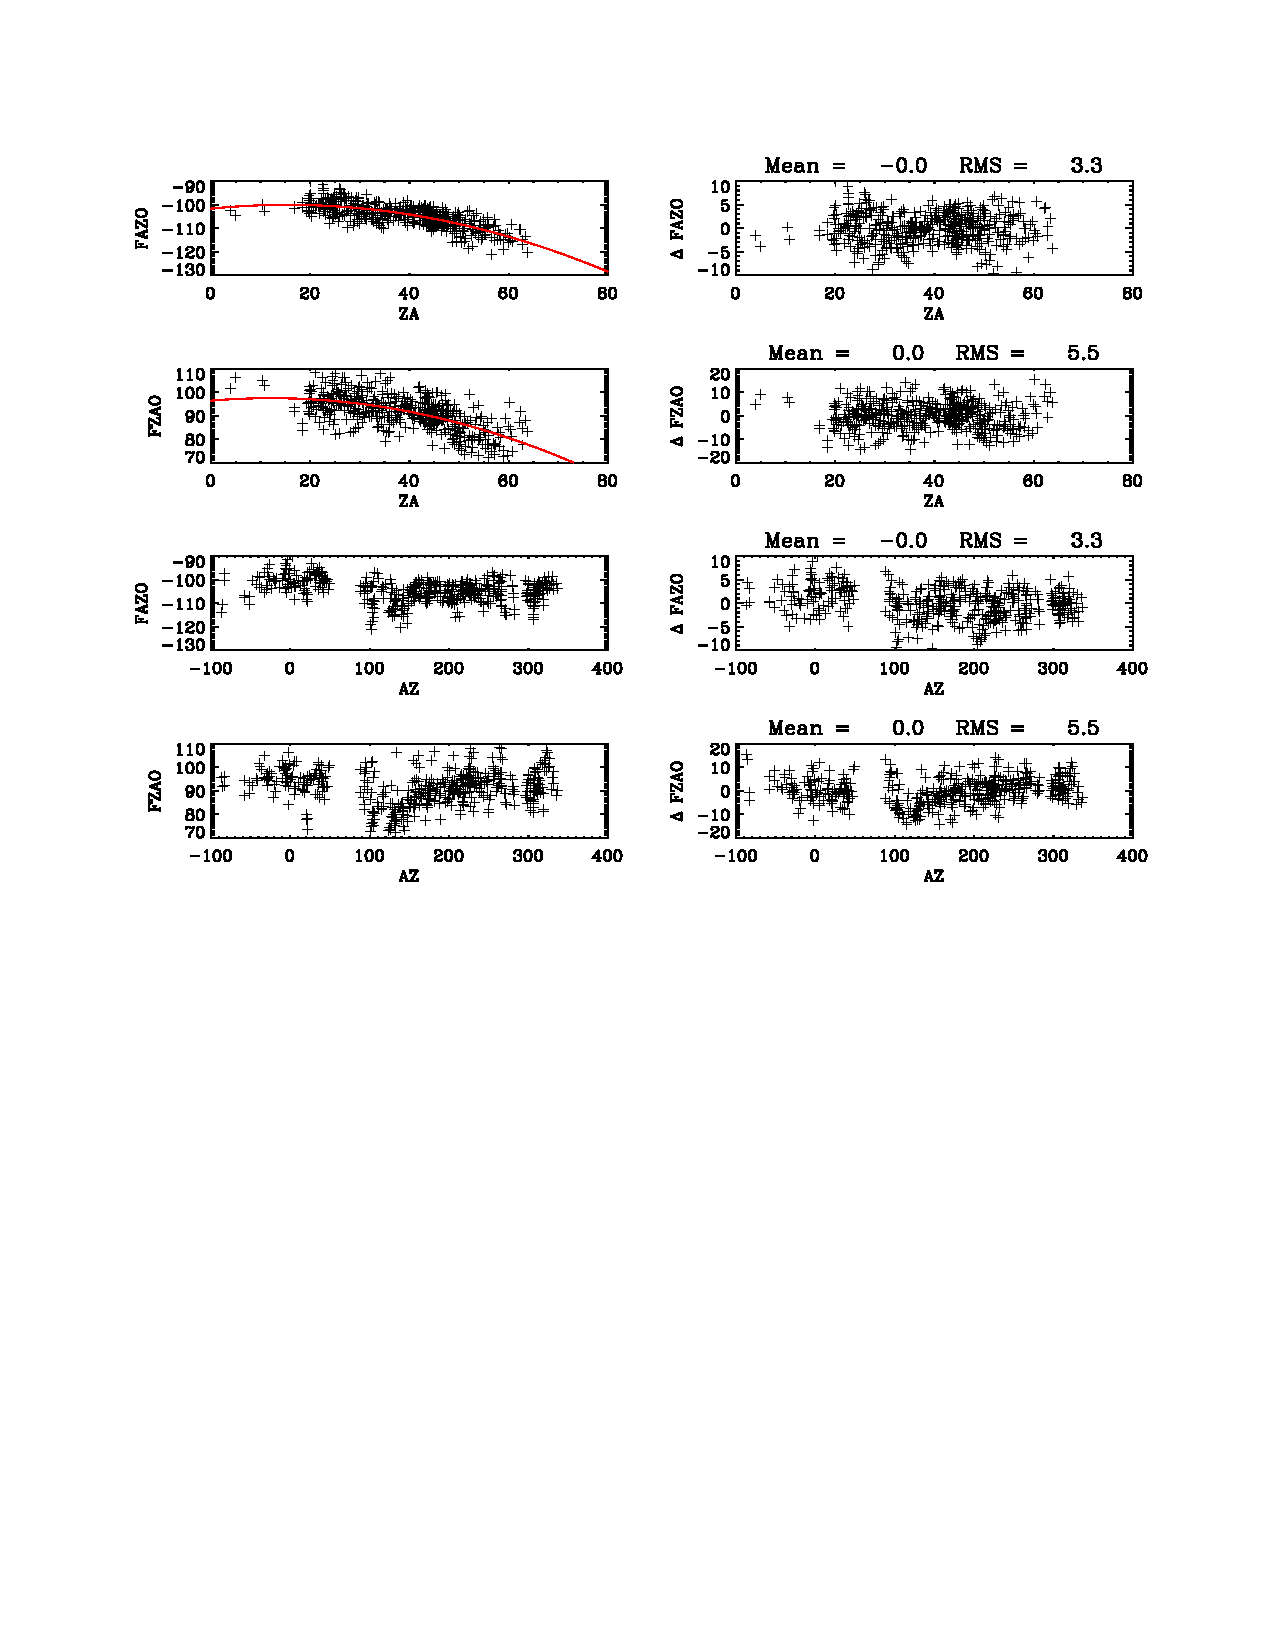
\includegraphics[scale=1.0]{pointing_model}}\\

  \subfigure[The residuals of the pointing model.  Note the Gaussian
distribution.]
{\label{fig:PointingModel-b}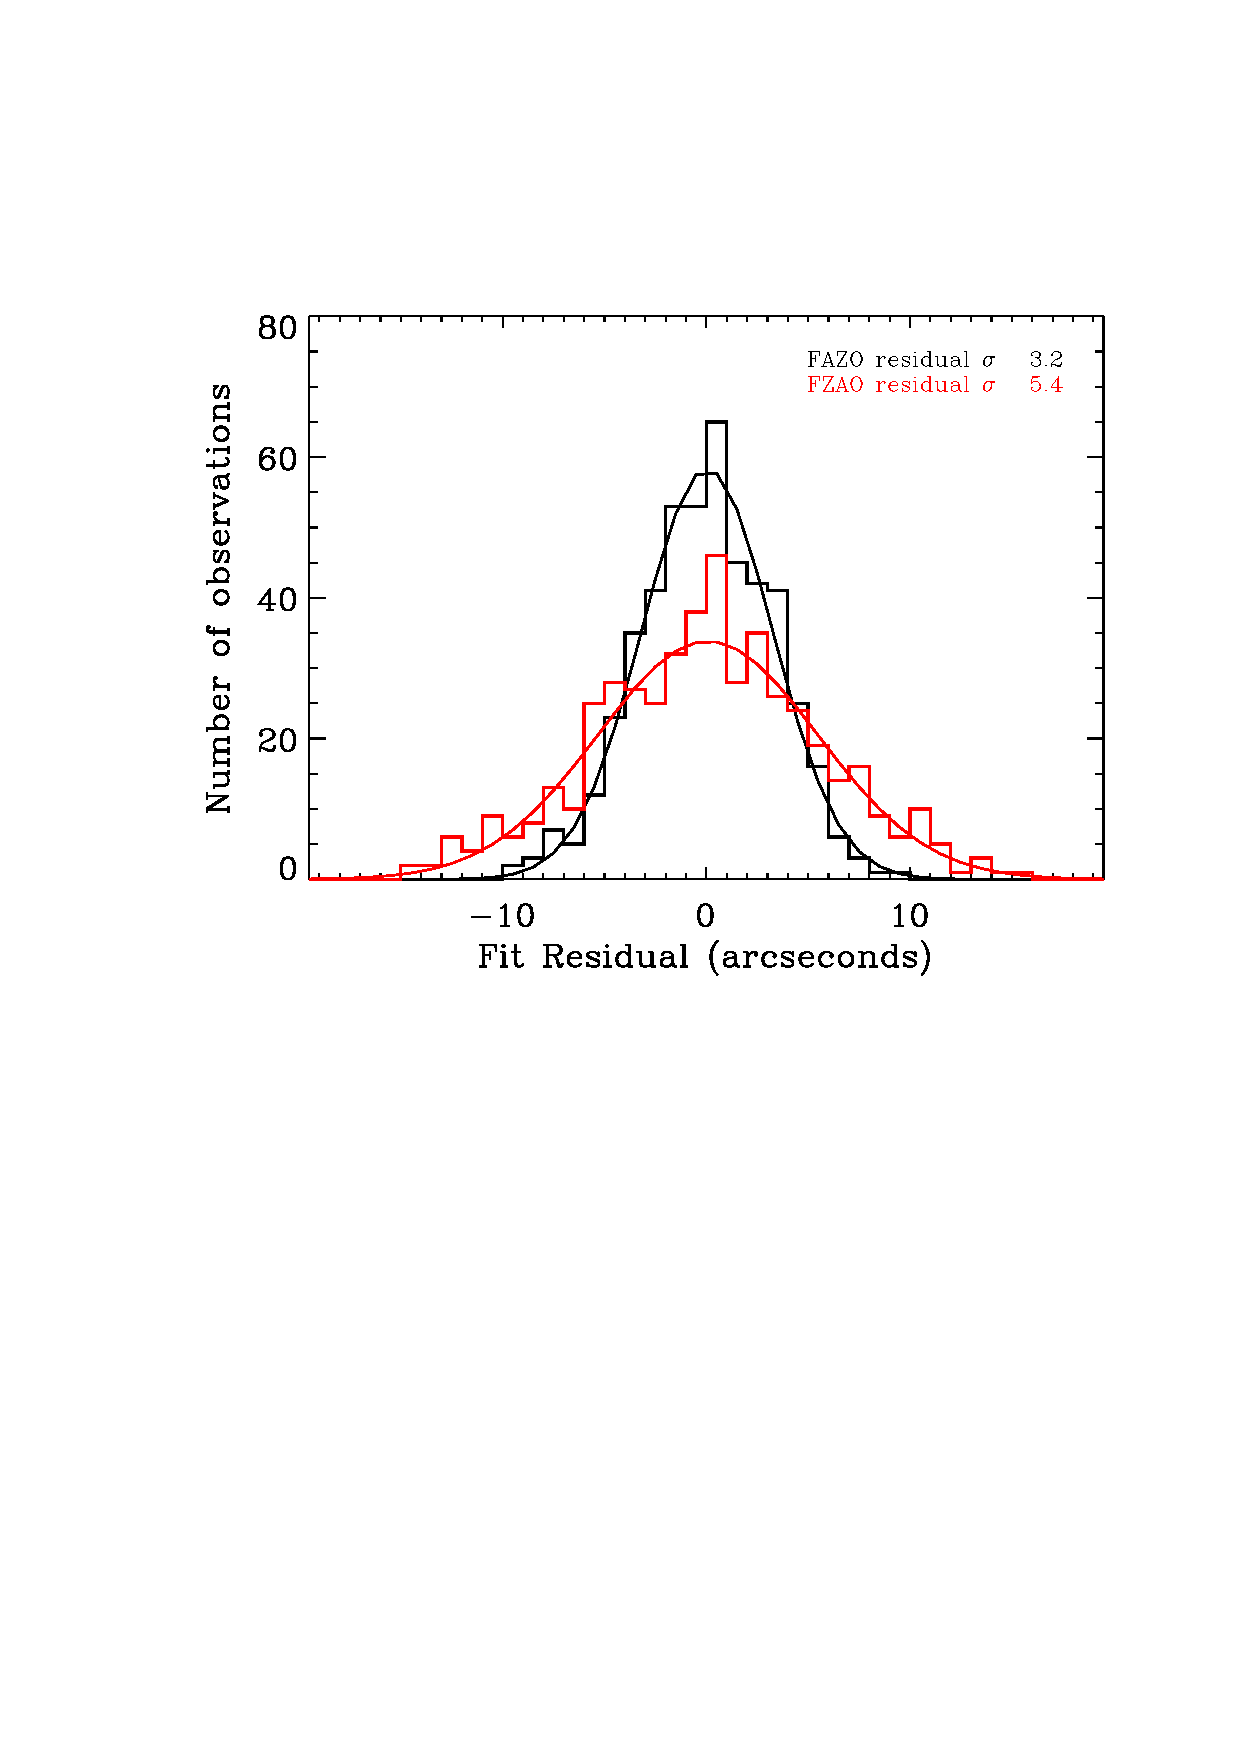
\includegraphics[scale=0.5]{pointing_model_residuals}}

\caption{The Bolocam pointing model for Epoch V.}
\label{fig:PointingModel}
\end{figure}
% -----------------------------------------------------------------------------


% 10
% -----------------------------------------------------------------------------
\begin{figure}

  \subfigure[{\it Left}: the Bolocam map in a portion of the $l=30$
  field.  {\it Right}: the SLC maps in the same region.  The green
  contours on the Bolocam map indicate the positions of the SLC
  sources.  \TBD\ {\it Do the negative bowls of either survey bunge up
  the cross-correlation?  If not, how do we deal with them?  The SCUBA
  image here has been somewhat doctored because of a large DC offset
  in the diagonal filament at center}]
  {\label{fig:SCUBAPointingComparison-a}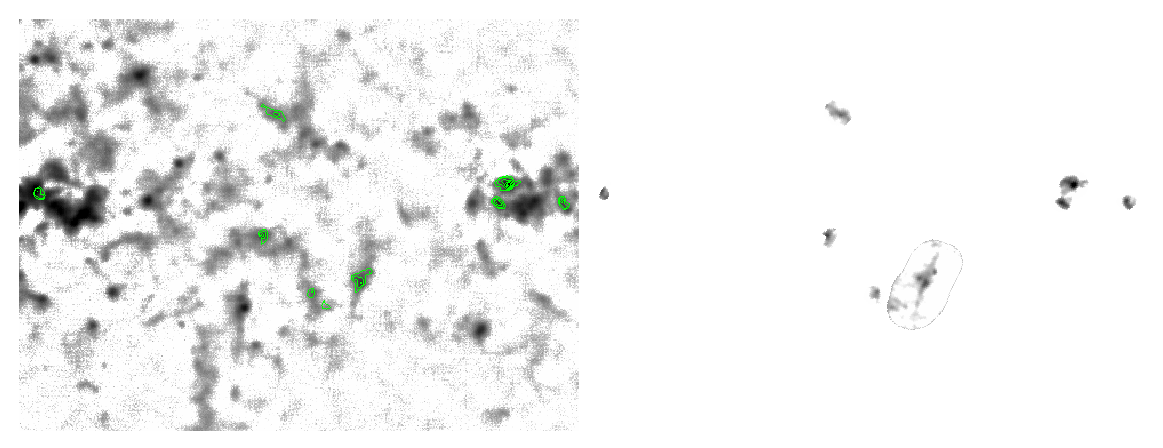
\includegraphics[scale=0.8]
  {scuba_bolocam_l030}}

  \begin{tabular}{cc}

  \subfigure[The cross-correlation map of the BGPS and SLC maps in
  Figure \ref{fig:SCUBAPointingComparison-a}. {\bf to be replaced with
  correct map}]
  {\label{fig:SCUBAPointingComparison-b}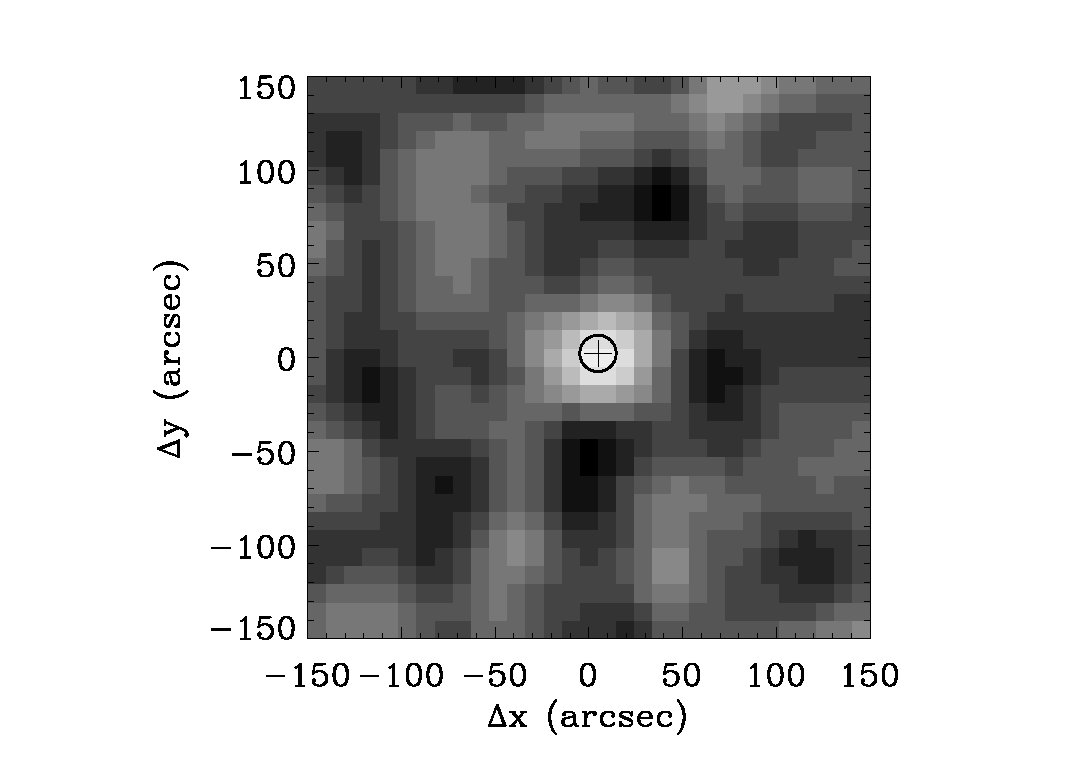
\includegraphics[scale=0.45]
  {xcorr_standin}}

  \subfigure[The measured offset between Bolocam and SCUBA Legacy
sources \citep{difrancesco08}, using the method described in Setion
\ref{sec:SCUBAPointingComparison}.  The circle indicates the $1\sigma$
region, which is also consistent with the error derived from the
internal Bolocam pointing model.]
{\label{fig:SCUBAPointingComparison-c}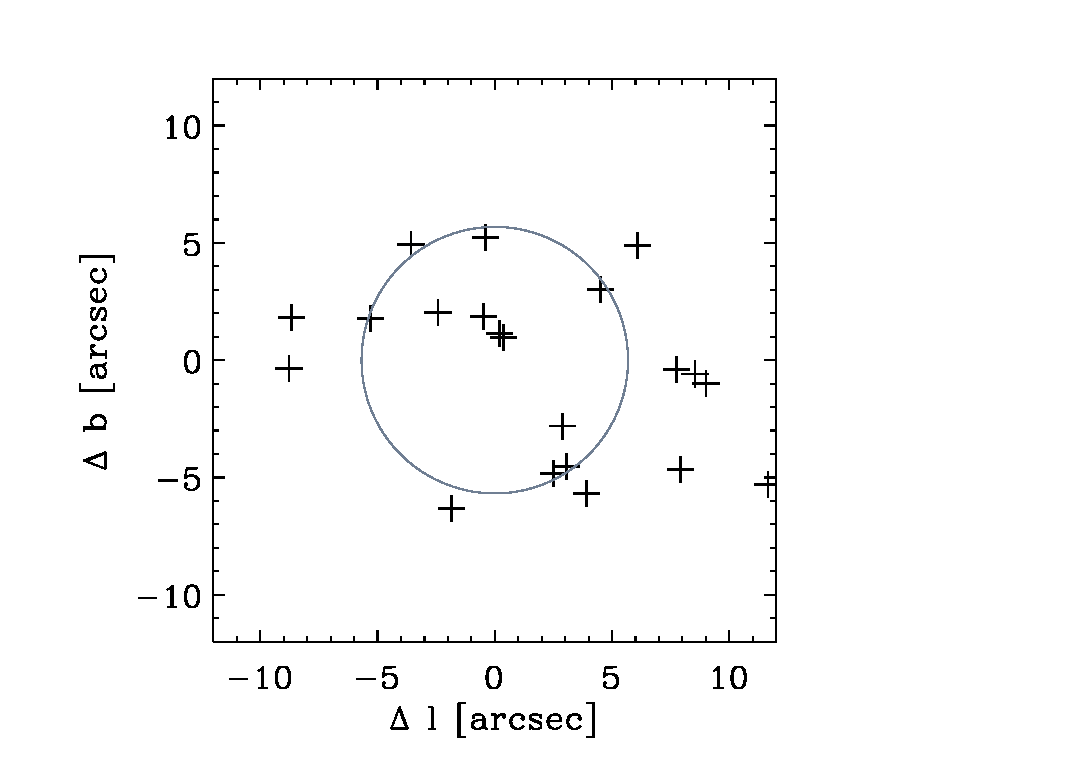
\includegraphics[scale=0.45]
{scuba_pointing_offsets}}

\end{tabular}

\caption{Comparing the Bolocam positions to those of the SCUBA Legacy Catalog.}
\label{fig:SCUBAPointingComparison}
\end{figure}
% -----------------------------------------------------------------------------

\section{Mapping Algorithm}
\label{sec:Mapping}

The essential signal-processing problem to be solved by the mapping
algorithm is the estimation and removal of a signal due to fluctuating
atmosphere emission which is $>\sim$100's of times stronger than the typical
sources in our maps.  We implement an iterative procedure for
estimating both the atmosphere fluctuations and the astrophysical
signal without {\it a priori} knowledge of either. 

We assume the raw timestream data $d$ for each bolometer (indexed by
$i$) can be written as
\begin{equation}
d_i(t) = s_i(t)+a_i(t)+e_i(t)+\epsi_i(t)
\end{equation}
where $s$ is the astrophysical signal, $a$ is atmospheric fluctuation
noise, $e$ are non-random signals due to the instrument itself, and
$\epsi$ is irreducible Gaussian noise due to photon shot and detector
noise.  The process of making a maximum likelihood map in the presence
of Gaussian noise is well-understood, and if the only contributions to
the data were $s$ and $\epsi$, then the minimum variance estimator of
the true astrophysical map is given by
\begin{equation}
\label{eq:LSMap}
m = (A^T W A) A^T W d
\end{equation}
where $A$ encodes the pointing information and $W$ is the inverse of
the covariance matrix of the time domain noise $\epsi$,
\begin{equation}
W = {\langle \epsi_i \epsi_j \rangle}^{-1}
\end{equation}
In this case, the mapping from data to map is a linear operator, $M
=(A^T W A) A^T W$.  For compactness, Equation \ref{eq:LSMap} will be
written as $M[d] = m$.  Note that the mapping operation is not
invertible.  However, given a map $m$ and an observing matrix $A$,
there exists a linear operation which makes predictions about the
observed timestreams, namely $d = A m$; this will be denoted $T[m] =
d$.

The goal is to produce a time series for each bolometer which as
closely as possible approximates $s + \epsi$ so that we may produce
the best estimate of the astrophysical signal $m = M[s+\epsi] = S + N$.

We proceed iteratively, estimating $a$ and $e$ in the order of their
relative strengths, beginning with the atmosphere.  The first
iteration step is then
\begin{equation}
\label{eq:FirstIterStep}
\tilde{a}^{(n)}(t) = 
\sum_i{d_i(t)-\tilde{s}^{(n)}_i(t) - \tilde{e}^{(n)}_i(t)}
\end{equation}
where $\tilde{s}^{(0)}_i(t)=0$.  This mean atmosphere model is then
fit to each bolometer to obtain the relative gains (flat field) of the
detectors
\begin{equation}
\tilde{a}^{(n)}_i(t) = \frac{d_i(t) \cdot a(t)}{d_i(t)^2} a(t) = r_i a(t)
\end{equation}
This is illustrated in Figure \ref{fig:Flatfield}.  The instrument
errors, which are typically smaller than the atmosphere, are then
estimated
\begin{equation}
\tilde{e}^{(n)}_i(t) = some models
\end{equation}
and both the atmosphere and instrument models are subtracted from the
raw time series
\begin{equation}
d_i(t) - \tilde{a}^{(n)}_i(t) - \tilde{e}^{(n)}_i(t)
\approx s_i(t) + \epsi_i(t)
\end{equation}
This is the best estimate of signal plus irreducible noise at
iteration step $n$, and is made into a map
\begin{equation}
M[d_i(t) - \tilde{a}^{(n)}_i(t) - \tilde{e}^{(n)}_i(t)] = \tilde{m}^{(n)}
\end{equation}
The current best map $\tilde{m}^{(n)}$ is then deconvolved to provide
a relatively low-noise, smooth map from which to generate a timestream
\begin{equation}
T[{\cal D}[\tilde{m}^{(n)}]] = \tilde{s}^{(n)}_i(t)
\end{equation}
where ${\cal D}$ represents the deconvolution operation.  At this
stage, the iterative process could begin again with Equation
\ref{eq:FirstIterStep}, though it is highly useful to produce an
``error map''
\begin{equation}
E = M[d_i(t) - \tilde{s}^{(n)}_i(t) - \tilde{a}^{(n)}_i(t) - 
\tilde{e}^{(n)}_i(t)]
\end{equation}
This error map serves as a straightforward visualization of the
progress of the iterative method, since in a perfect process it would
be map of $\epsi$.

\subsection{Atmosphere Fluctuation Noise Model}

The simplest model for the atmosphere fluctations makes use of the
fact that the beams for all of the detectors pass through a nearly
identical atmosphere, thus implying that atmosphere fluctuations will
be highly correlated between detectors.

To further remove the atmosphere (and other correlated instrument
noise) without a detailed physical model, we use a principal component
analysis (PCA) as given in \citet{laurent05}.


\subsection{Instrument Error Signals}

Most of the instrument error signals have characteristic features
which allow them to be identified, though not always removed.  The
error signals include the following:
\begin{enumerate}

\item Pickup from the 60 Hz AC power.  This appears as narrow lines in
the PSD of the data.  The second harmonic of 60 Hz is aliased via
beating against the 130 Hz bolometer bias frequency into 10 Hz with
sidebands split at $\sim1$ Hz.

\item Spikes in voltage due to cosmic ray strikes on the bolometers
(``glitches'').

\item Microphonic pickup due to vibrations of the receiver.  The most
noticeable microphonics occur at the end of each scan when the
telescope is turning around and the field rotator is adjusting.  This
leads to broad spikes in the time series, whose long decay must be
removed from the data, particularly during the beginnings of scans.

%\item Others?

\end{enumerate}

Fortunately, most of the AC powerline pick-up occurs at frequencies
where there is no astrophysical signal, given the beam size and scan
speed.  Thus this error is dealt with by first notch filtering at the
line frequencies and then low-pass filtering the data.  Because of the
low correlation with astrophysical signal, this step is performed only
once and is not iterated (c.f. Figure XXX of \citet{sayers09}).

Both glitches and microphonic pickup from the scan turnarounds are
degenerate with astrophysical signal and must be estimated as part of
the iterative process.  Glitches are identified as large excursions
from the RMS level after subtraction of the best atmosphere and bright
source model, and the data there is excluded from inclusion in
subsequent maps.  The turnaround microphonics are modeled as decaying
exponentials at the beginnings and ends of scans.

\subsection{Data Flagging}

Due to the large volume of data generated by the survey, it was
necessary to develop new tools to quickly visualize the data and
ensure data quality.  A common tool in radio astronomy is the
so-called ``waterfall'' plot, which is an image with frequency on the
x-axis, time on the y, and an intensity proportional to the
interferometer visibility amplitude or phase.  We have used a variant
on this to visualize the Bolocam data by displaying bolometer number
(related to the bolometer position in the focal plane) on the x-axis
and time on the y, with the intensity given by the bolometer's
response (in Jy) at that time.  An example of this is shown in Figure
\ref{fig:Flagger}.  With practice, anomalies such as the glitch shown
can be detected and manually and iteractively flagged out.

An automated flagger was also created that flags out outlier data on a
per-pixel basis.  In order to make a robust measurement of the
variance of the fluxes assigned to each pixel, we used the median
average deviation (MAD) over the data in the pixel and rejected high and low
outliers at the 3-sigma level.  Pixels with too little data to compute
a deviation, i.e. those with $<3$ data points, were also flagged out -
these scan-edge pixels are the dominant contribution to the total
number of flagged data points.

\subsection{Creation of the Astrophysical Model}

%WRITTEN POORLY: 
The timestream data is made into a spatial map using the pointing data
corresponding to each time point for each bolometer.  The data is
weighted by inverse variance across a single scan and then drizzled
into a map with $7.2$\arcsec\ pixels using a nearest-neighbor
algorithm.  The nearest-neighbor matching allows the map to be
returned to a timestream in the same manner, but with the S/N improved
by averaging over all hits on a given pixel.  It has the disadvantage
that it accentuates the unevenness of the cross-scan sampling, since
ech timestream point's value is assigned to an area much smaller than
the beam.

The resulting map is then subjected to a Hogbom-type CLEAN algorithm
\citep{hogbom} using a specified kernel to produce a deconvolved
image.  This has several advantages over the 

\setcounter{subfig}{1}
\renewcommand{\thefigure}{\arabic{figure}\alph{subfig}}

\begin{figure}
  \begin{minipage}{6.5in}
    \begin{center}
      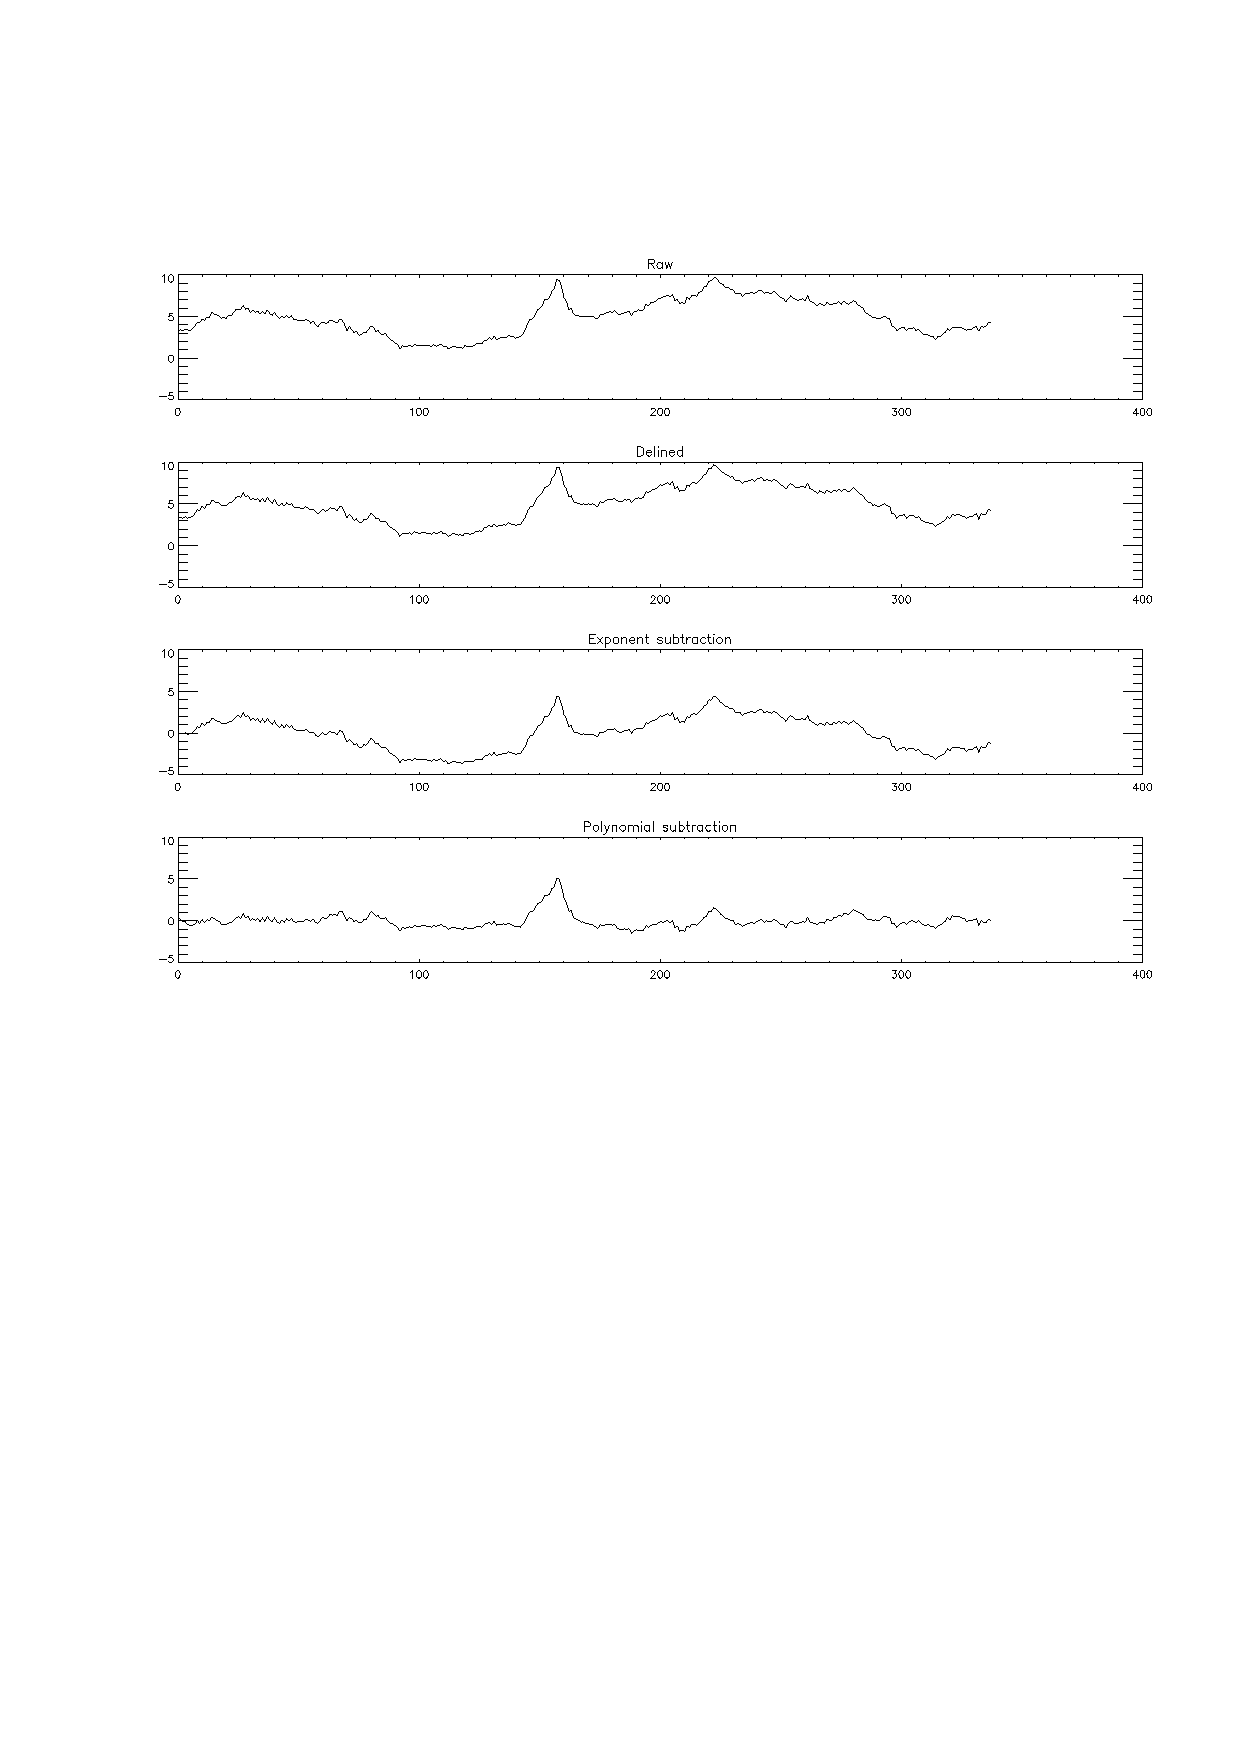
\includegraphics[scale=0.9]{iterative_mapping1}
      \caption{An example of the change in the time series as
      iterative mapping proceeds.}
    \end{center}
    \label{fig:IterativeMapping}
  \end{minipage}
\end{figure}

\addtocounter{figure}{-1}
\addtocounter{subfig}{1}

  
\begin{figure}
  \begin{minipage}{6.5in}
    \begin{center}
      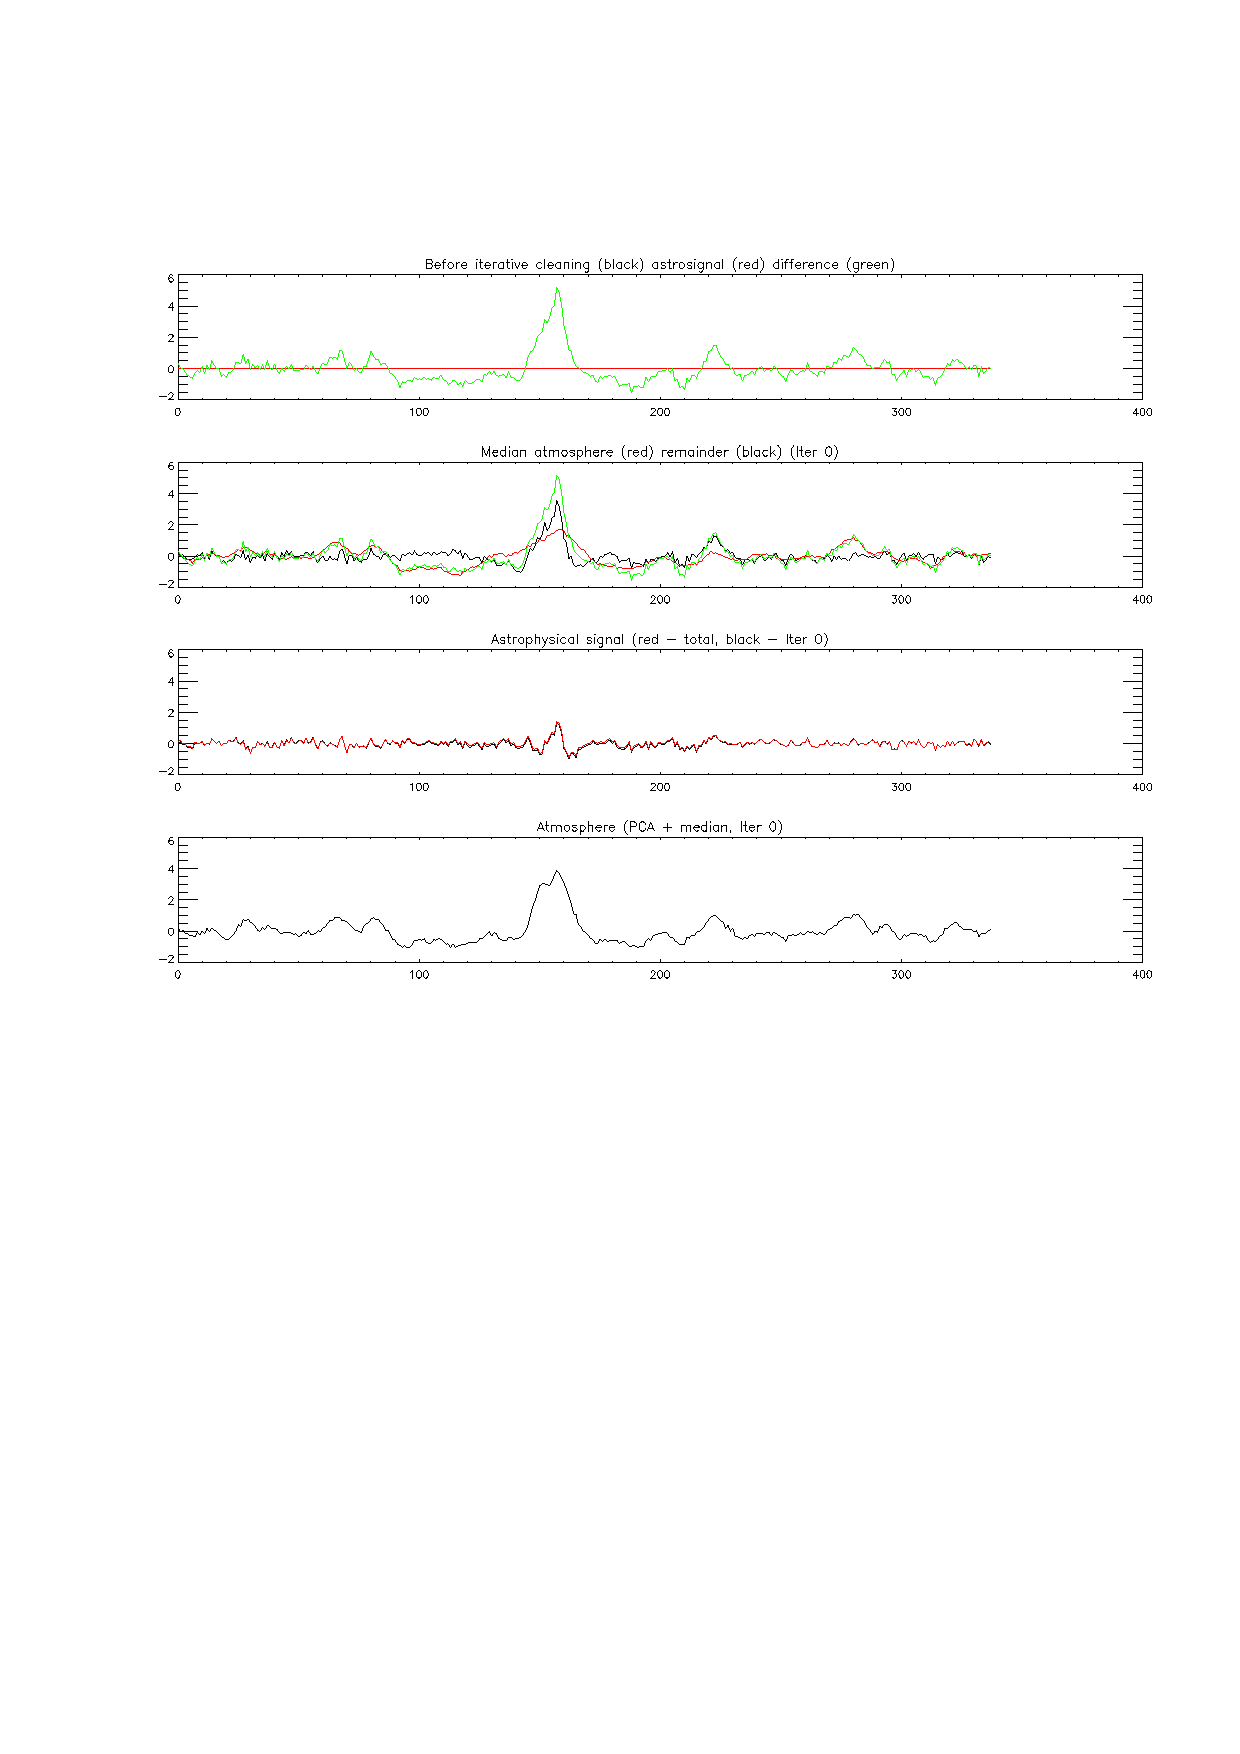
\includegraphics[scale=0.9]{iterative_mapping2}
      \caption{}
    \end{center}
    \label{fig:IterativeMapping-b}
  \end{minipage}
\end{figure}

\addtocounter{figure}{-1}
\addtocounter{subfig}{1}

\begin{figure}
  \begin{minipage}{6.5in}
    \begin{center}
      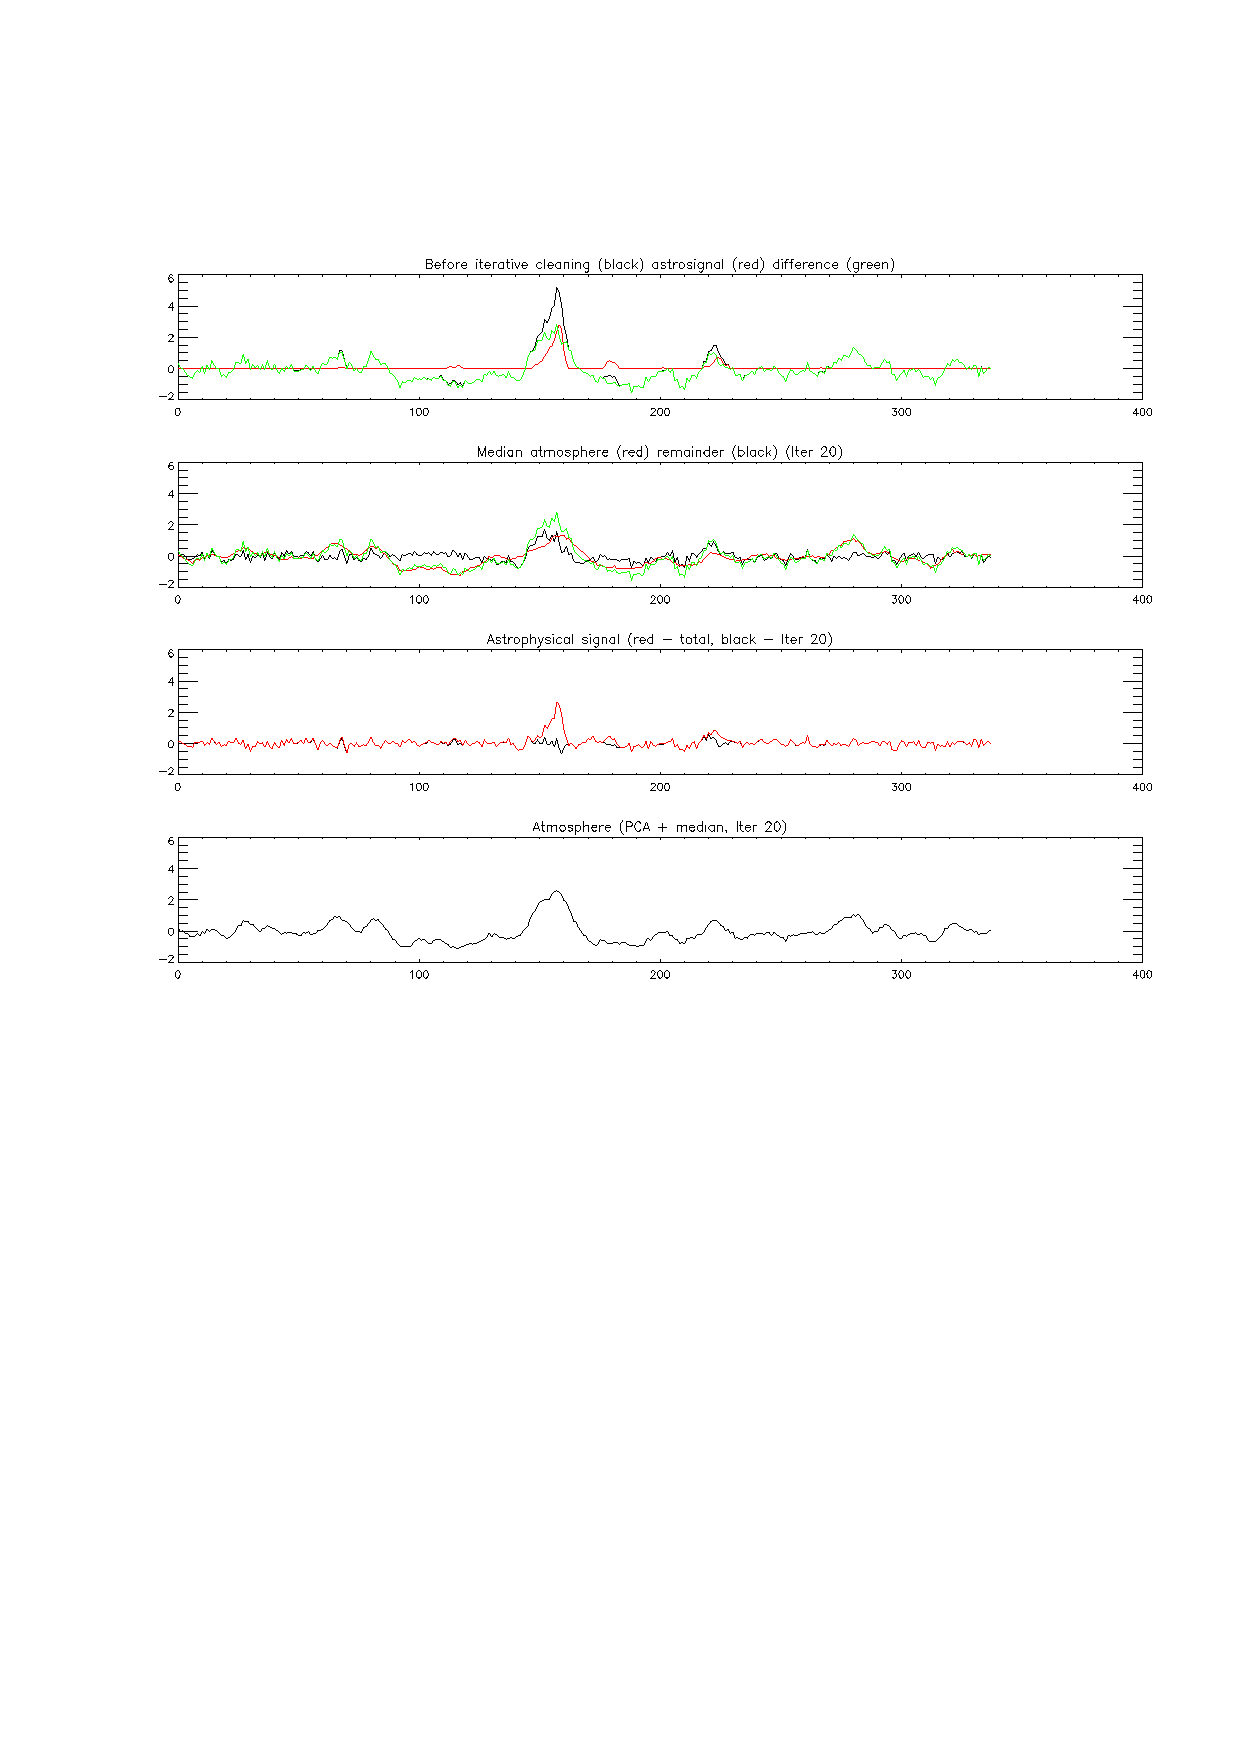
\includegraphics[scale=0.9]{iterative_mapping3}
      \caption{}
    \end{center}
    \label{fig:IterativeMapping-c}
  \end{minipage}
\end{figure}

% -----------------------------------------------------------------------------
\setcounter{subfig}{1}
\begin{figure}
  \begin{minipage}{3.25in}
    \begin{center}
      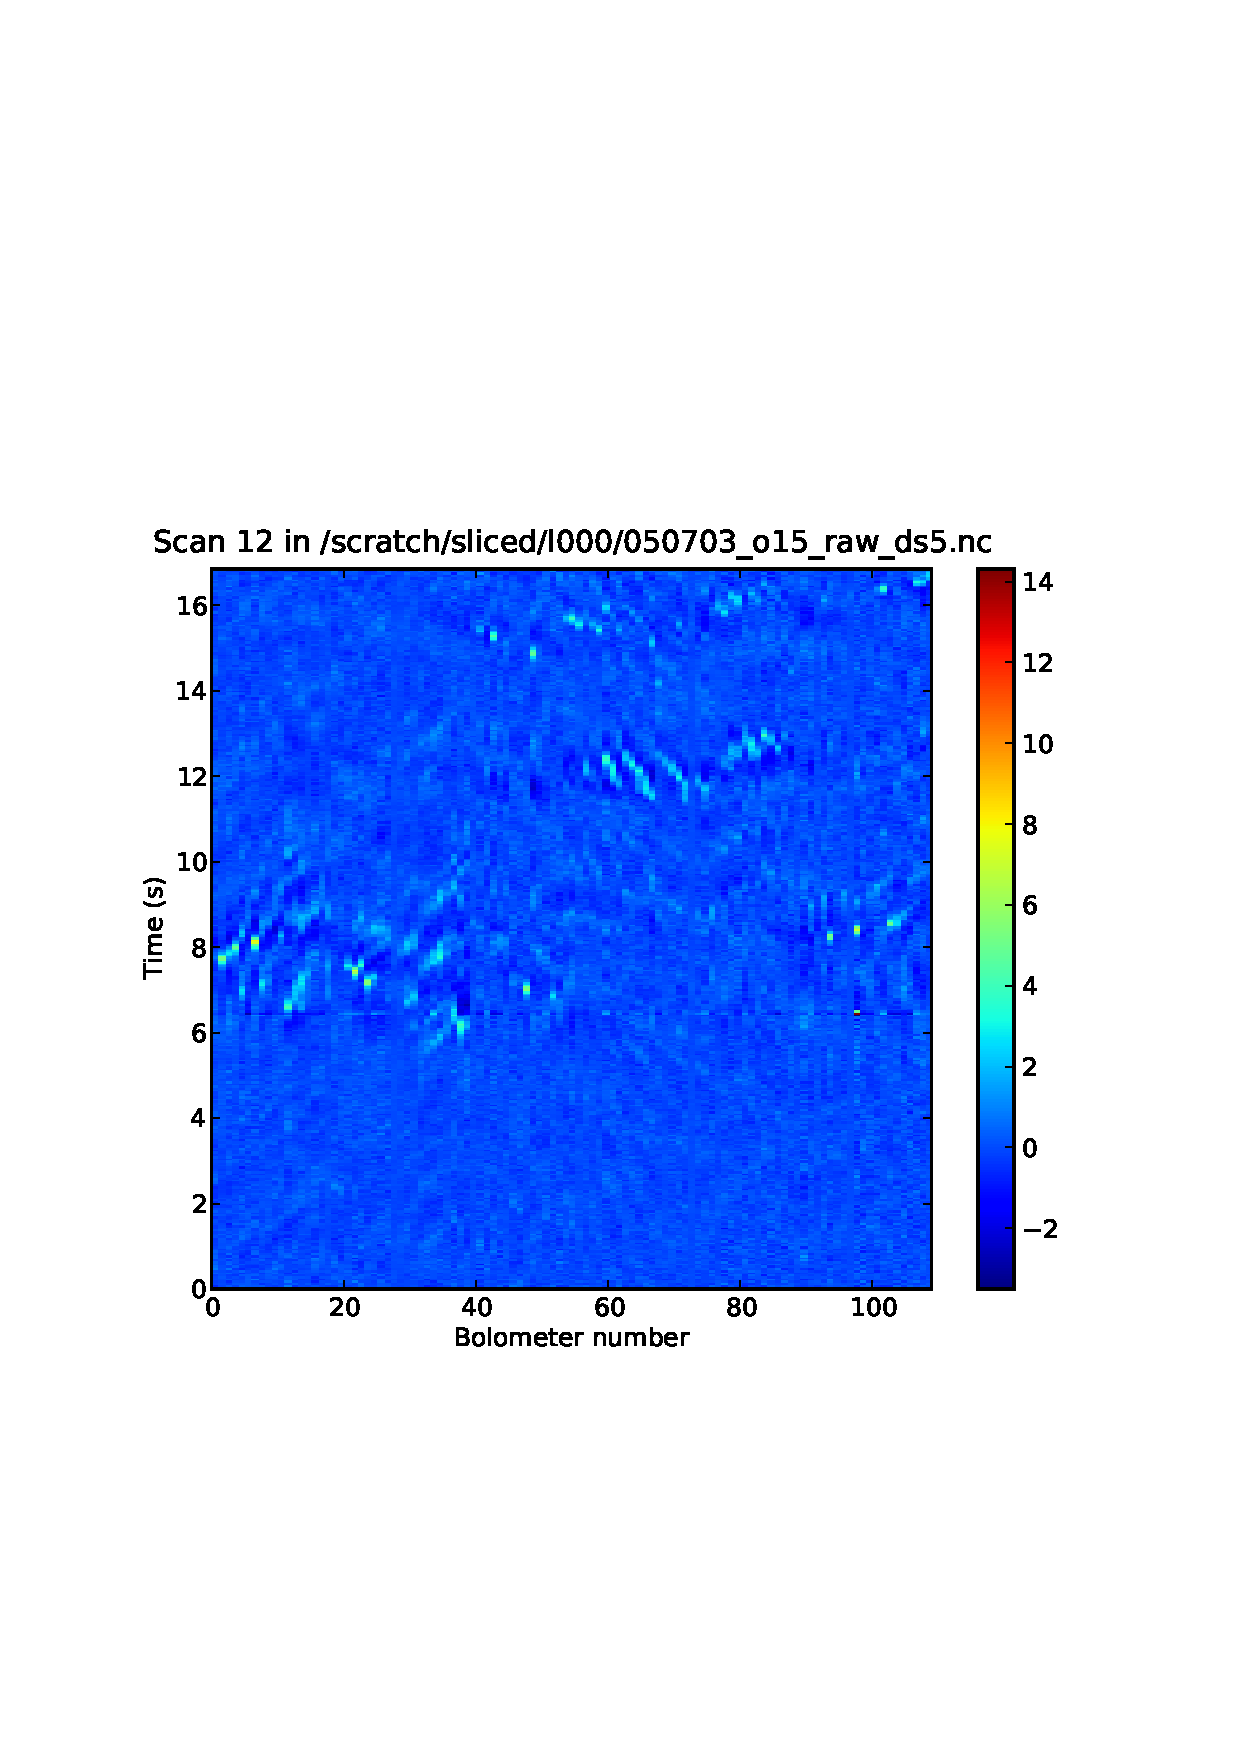
\includegraphics[scale=0.5]{flagger_withglitch}
    \end{center}
  \end{minipage}
  \begin{minipage}{3.25in}
    \begin{center}
      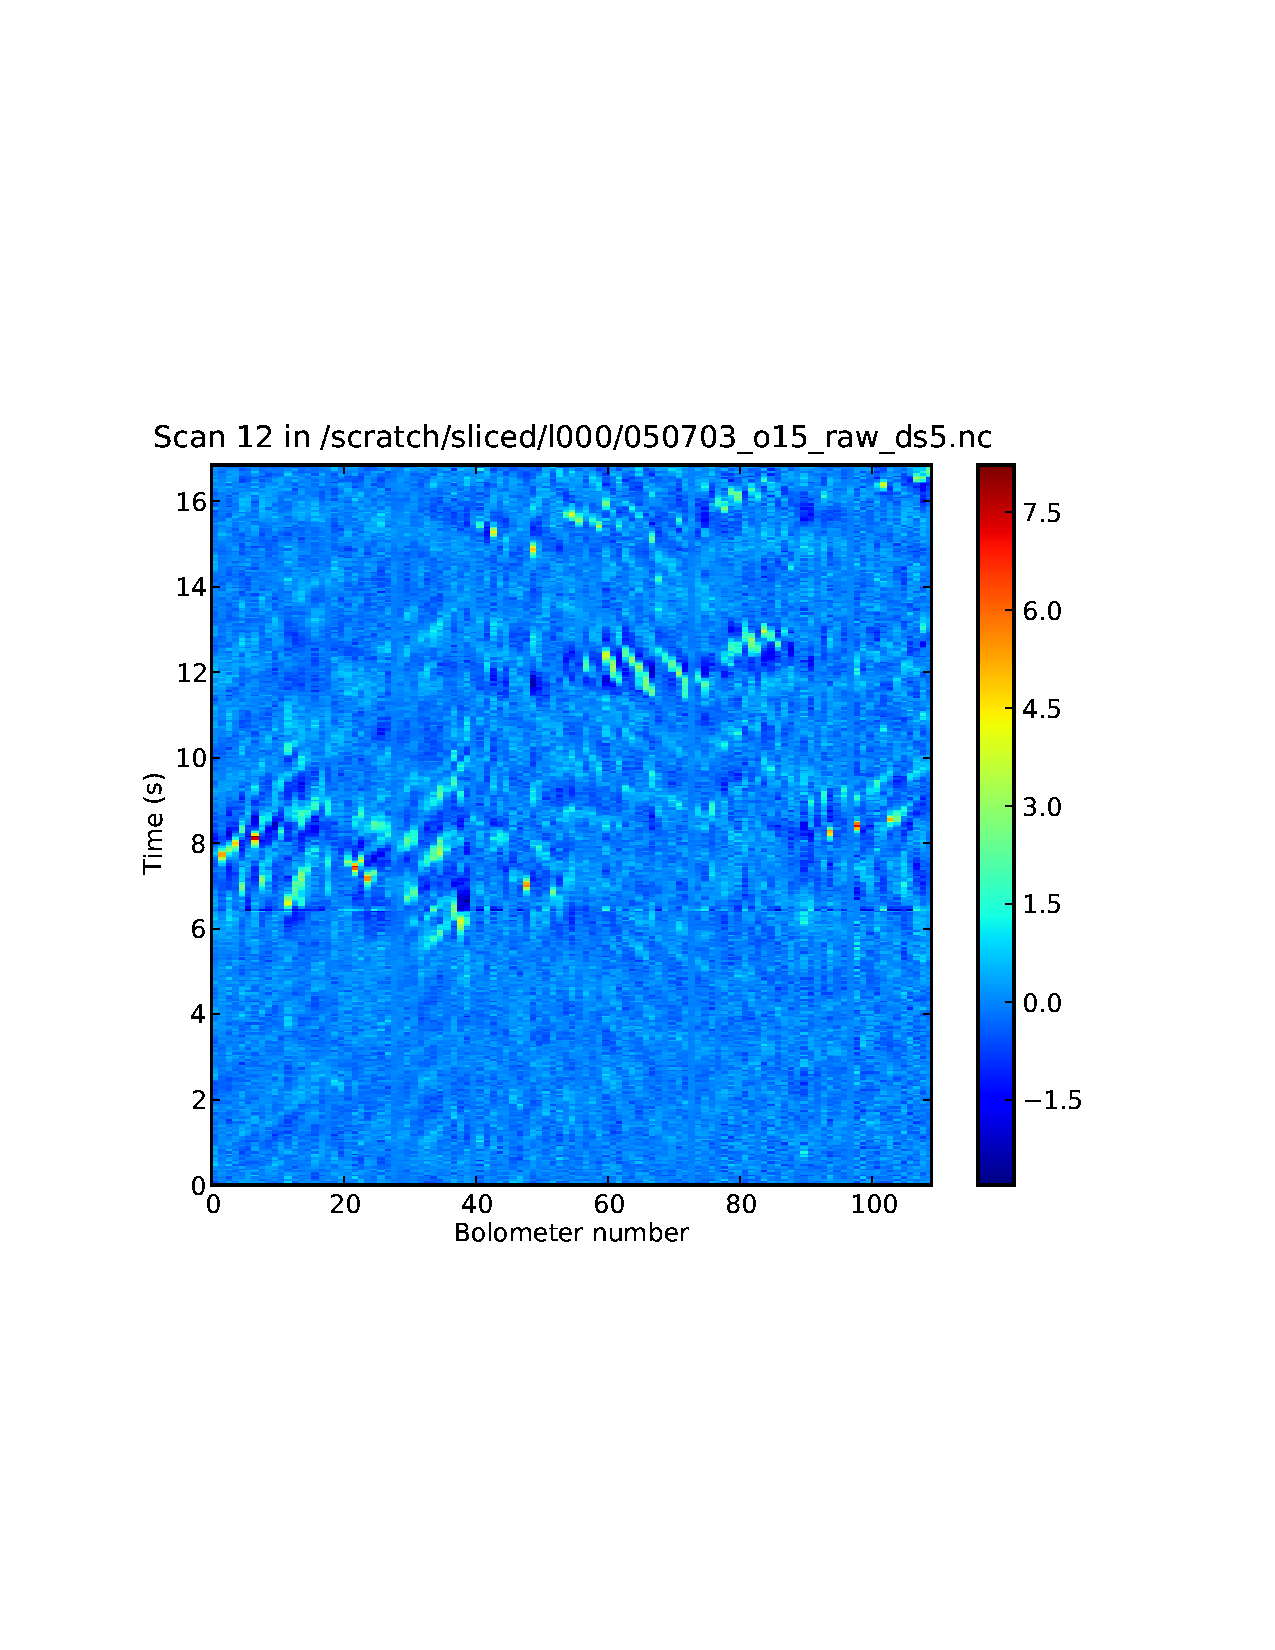
\includegraphics[scale=0.5]{flagger_glitchgone}
    \end{center}
  \end{minipage}
  \caption{An illustration of the flagging process using the waterfall
plot. Left: The glitch apparent at middle right is the same one whose
time series is shown in Figure \ref{fig:CosmicRayGlitch}.  Because of
the PCA subtraction, the effect of the glitch also propagates over the
other bolometers, appearing as a horizontal stripe. Right: The same
data displayed with the time point including the glitch flagged out
and rescaled}

  \label{fig:Flagger}

  \addtocounter{figure}{-1} 
  \addtocounter{subfig}{1}
  
  \begin{minipage}{6.5in}
    \begin{center}
      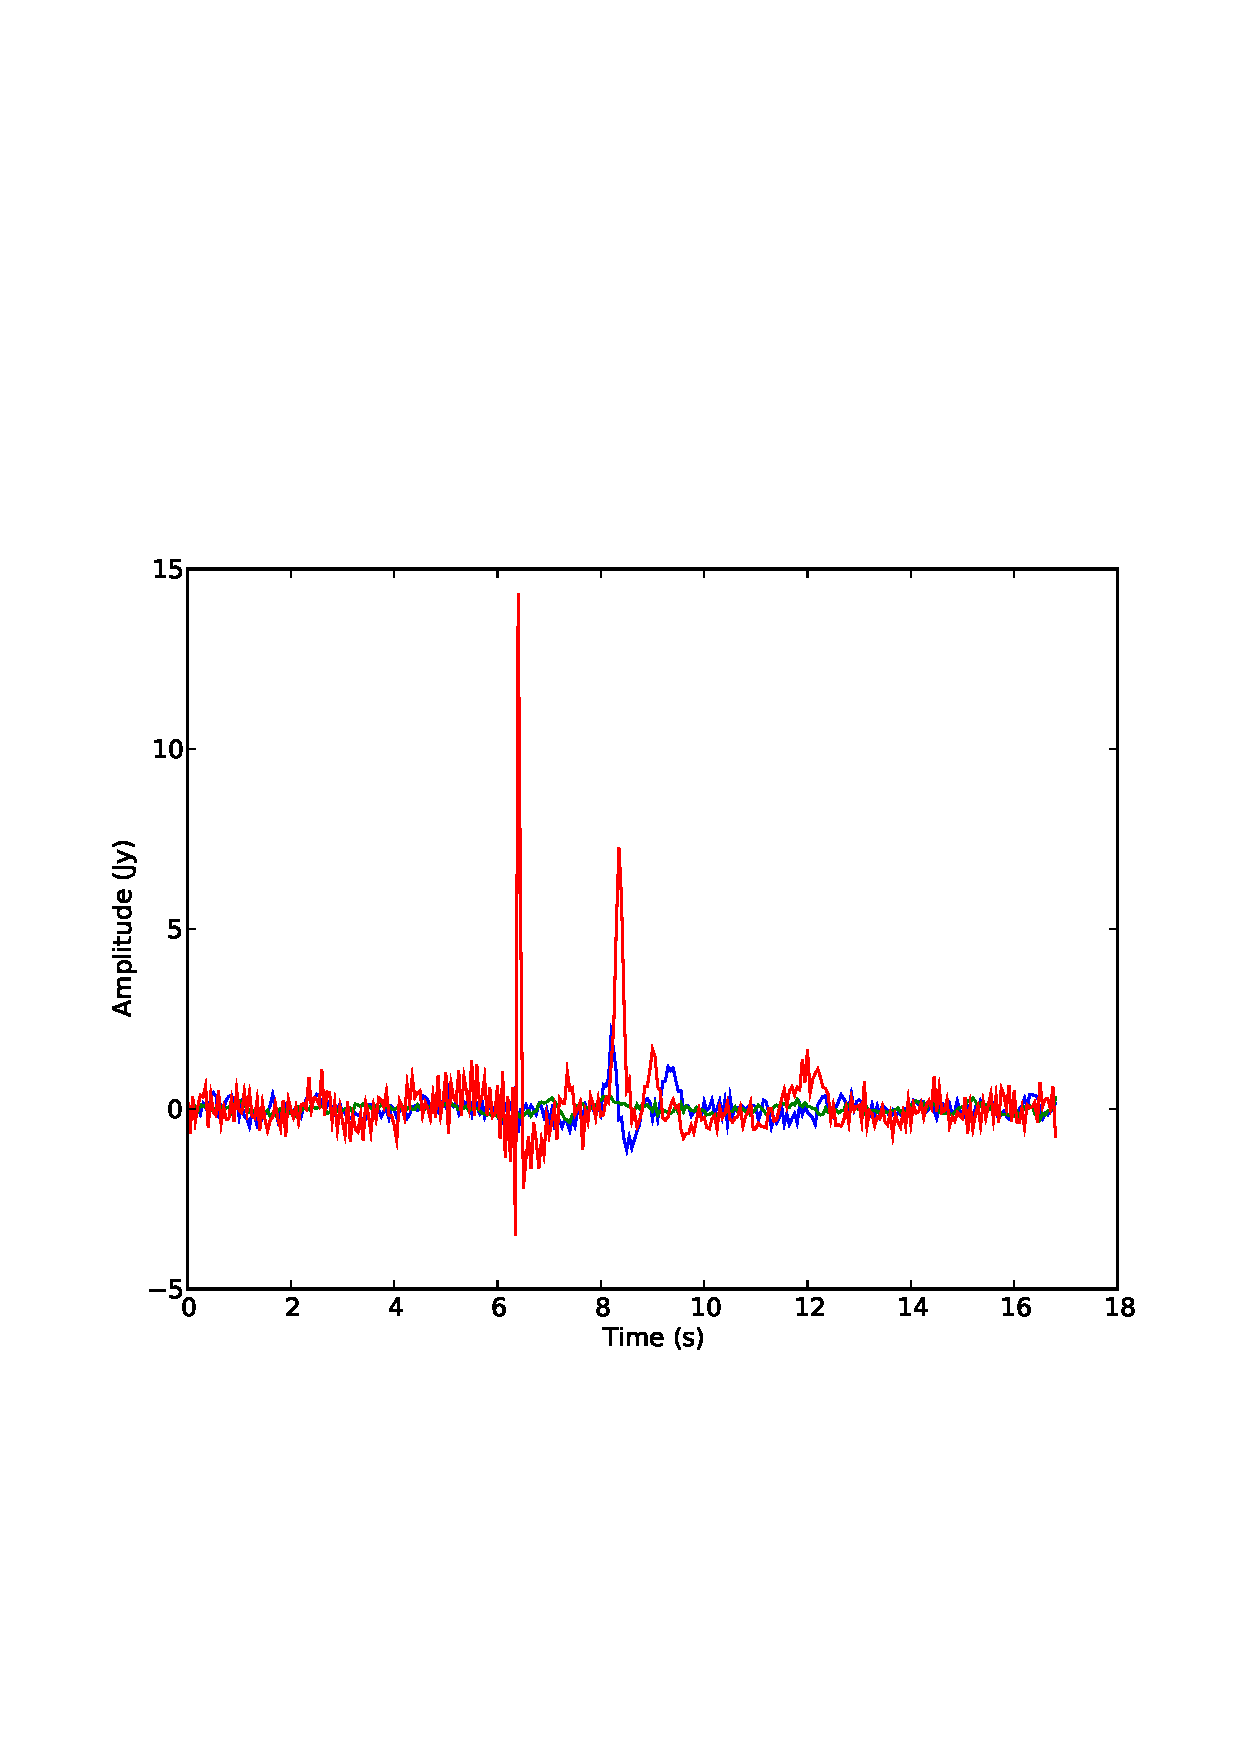
\includegraphics[scale=0.5]{flagger_plots}
      \caption{An illustration of a ``glitch'' in a single bolometer
timestream (red) due to a cosmic ray strike.  Note the acausal ringing
due to the application of the downsampling filter.  The time series
for a physically adjacent bolometer is shown in blue, and a bolometer
which does not pass over a source in green.  The PCA model has already
been subtracted from the data.}
    \end{center}
  \end{minipage}

\end{figure}

% -----------------------------------------------------------------------------

\renewcommand{\thefigure}{\arabic{figure}}



%\FigureTwo{flagger_withglitch}{flagger_glitchgone}{An illustration of
%the flagging process using the waterfall plot. Left: The glitch
%apparent at middle right is the same one whose time series is shown in
%Figure \ref{fig:CosmicRayGlitch}.  Because of the PCA subtraction, the
%effect of the glitch also propagates over the other bolometers,
%appearing as a horizontal stripe. Right: The same data displayed with
%the time point including the glitch flagged out and rescaled}
%{fig:Flaggin}{1.0}
%
\Figure{crs}{The distribution of glitch amplitudes flagged and removed
from the data.  The expected contribution to the noise from the
unremoved glitches below the detection threshold is
\TBD.}{fig:GlitchDistribution}{1.0}

\begin{figure}
  \begin{minipage}{6.5in}
    \begin{center}
      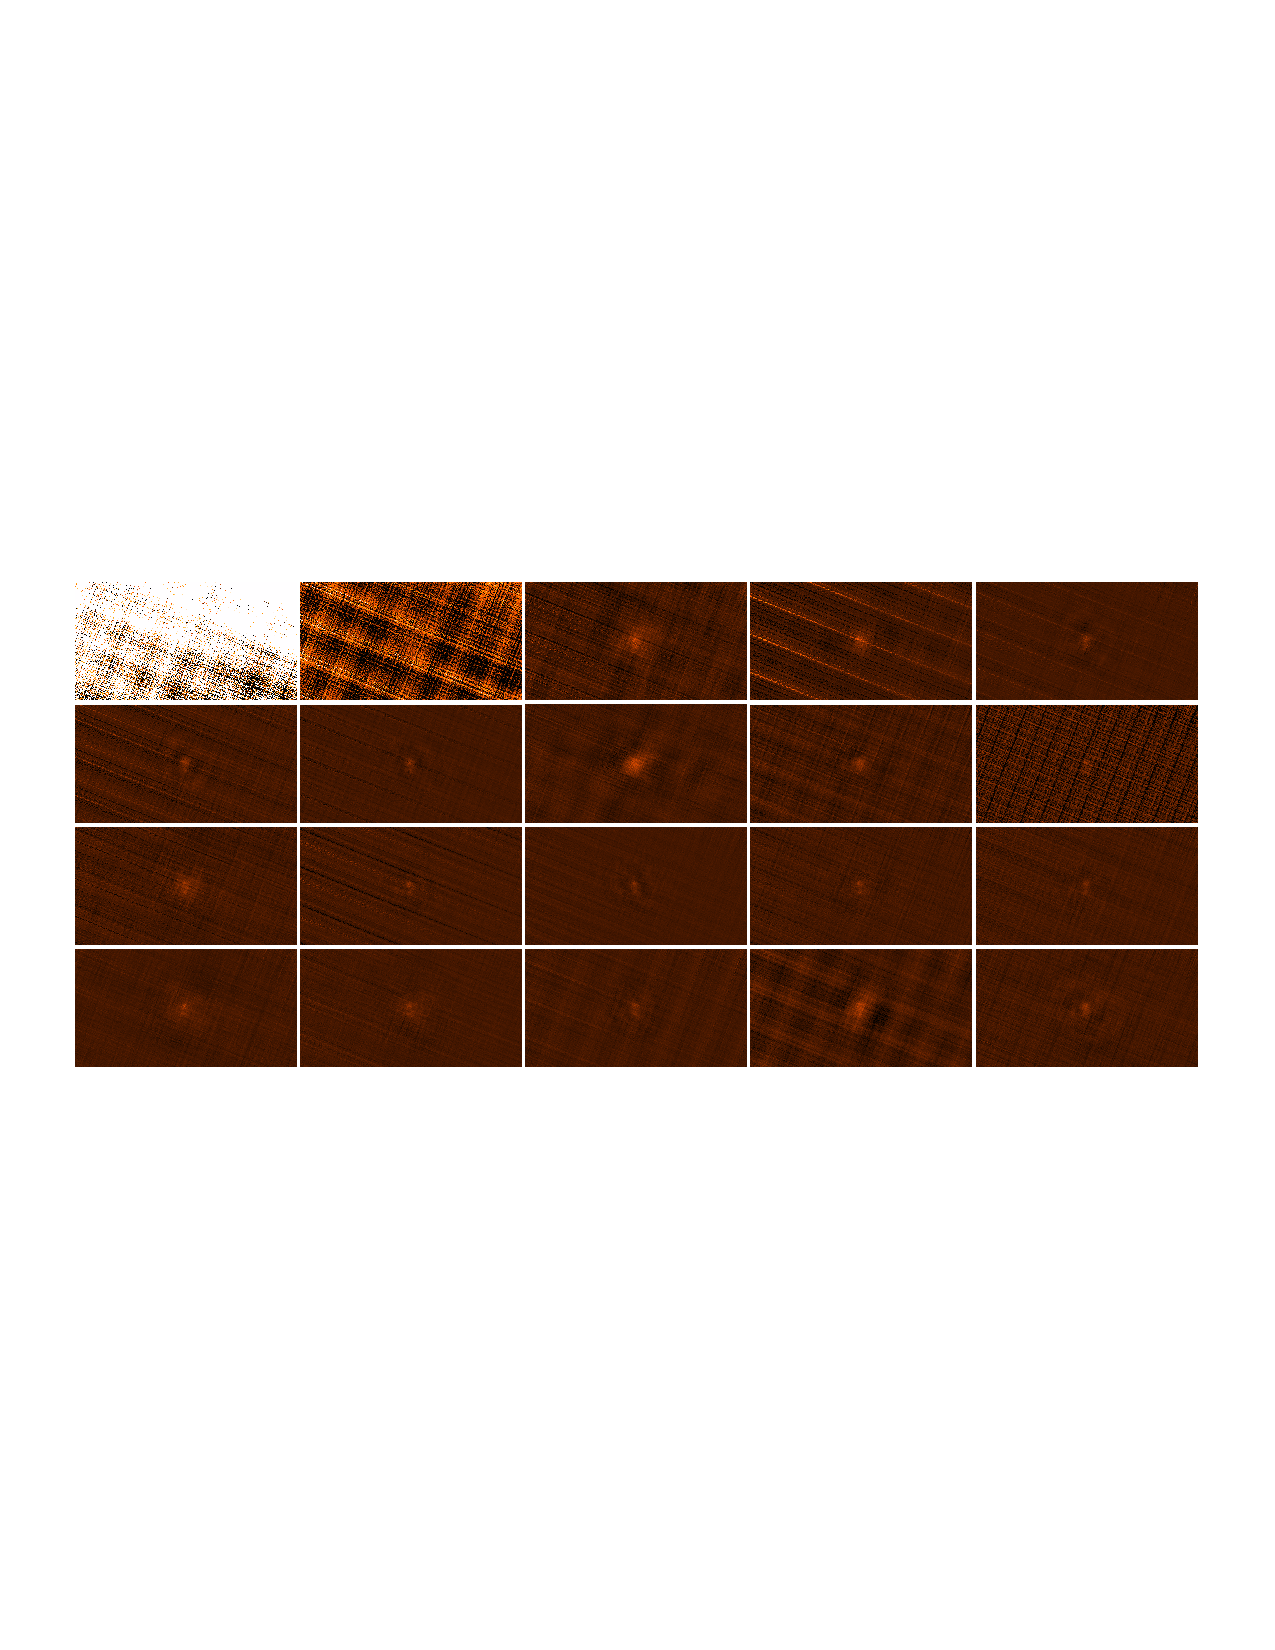
\includegraphics[scale=0.8]{eachpca}
    \end{center}
  \end{minipage}
\vspace{0.25in}
  \begin{minipage}{6.5in}
    \begin{center}
      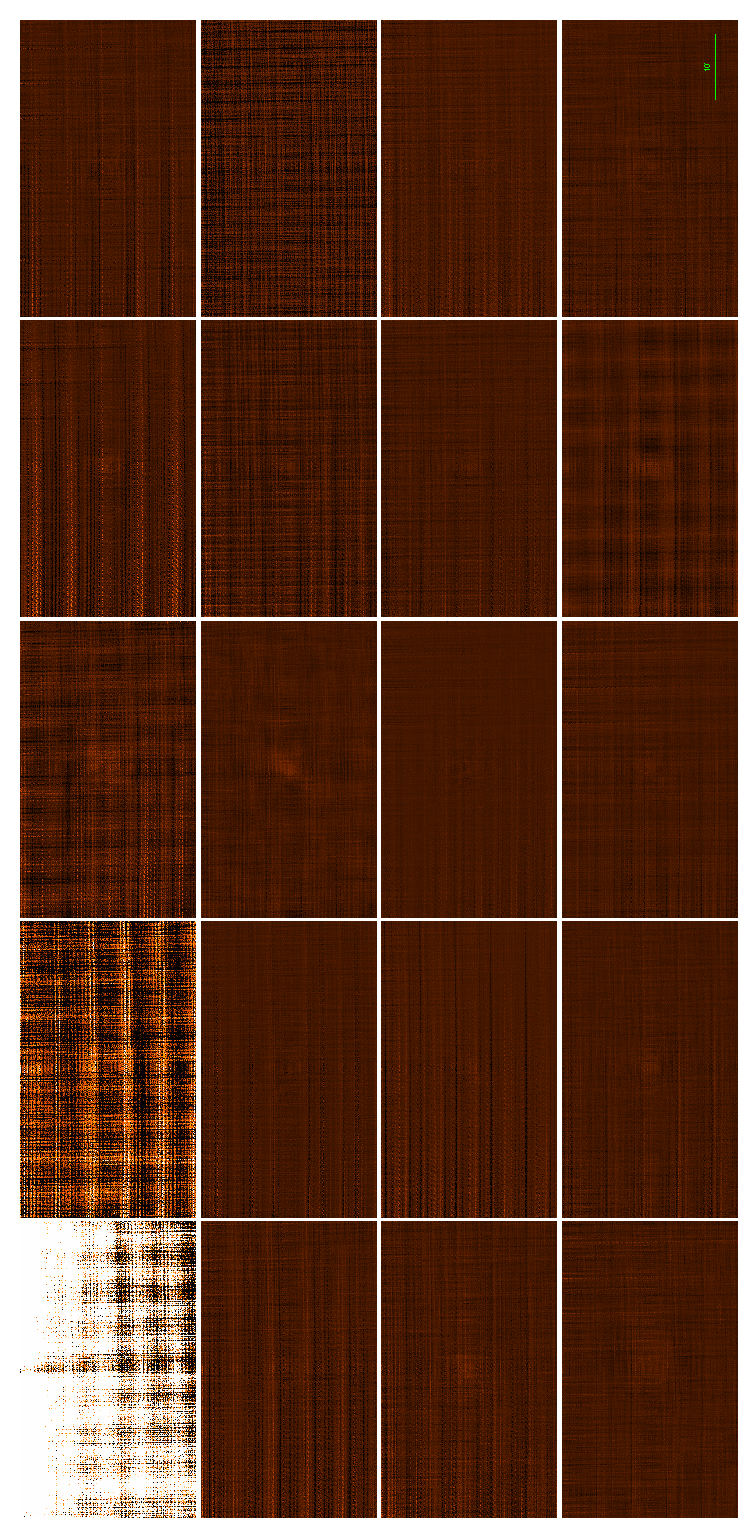
\includegraphics[scale=0.8]{eachpca_20iters}
    \end{center}
  \end{minipage}
  \caption{{\it Top}: a grid of maps of the first 20 PCA components
displayed at the same scale.  It is clear that NCG 7538, the object
imaged, has correlated emission in each component.  There are varying
levels of correlated noise in each component, with the first through
third being the most obvious atmospheric components.  Most of the
other noise components are probably various bits of correlated
detector noise. {\it Bottom}: The same figure, but after 20
iterations.  The figure is the breakdown of the atmosphere remainder
(i.e. the raw data minus the astrophysical model) into eigenfunctions.
Very little astrophysical flux remains at any level of correlation,
though there is some at large (few arcminute) scales.}
\label{fig:PCA_Graphical}

\end{figure}

\Figure{l001_deconvolutionkernelcompare}{The effect of deconvolution
on the iterative process can be seen in its effect on the
residuals. From left to right: map, noise, smoothmap, model. Top to
bottom kernel size: 14.4\arcsec, 21.6\arcsec, 31.2\arcsec,
7.2\arcsec. The final version of the pipeline uses 14.4\arcsec, which
has the result of leaving no flux in the residual at the location of
Sgr B2, and does not ``dig a hole'' in the residual map, as the
7.2\arcsec\ kernel does.}{fig:Deconvolution}{1.0}

\clearpage

\section{Noise and Systematic Effects}
\label{sec:Noise}

The error maps produced by the iterative mapping provide a natural way
of estimating the systematic error resulting from imperfect
subtraction of bright sources.  This results in ``ghosts'' of the
bright sources in the error maps $E$.  

% this is not true.  I can't do jackknifing....
% To estimate the size of this
% residual error, we also construct jackknife maps for each field, in
% which the astrophysical signal is made to exactly cancel.  This
% provides an estimate of the noise-only RMS in the maps, to which
% deviations from the ``ghosts'' may be compared.

In some fields, flux from certain source spread out over the course of
the iterative process using certain kernel sizes.  The cause of this
artifact are not yet well-understood, but using a different kernel
size was an effective workaround and did little to change the
properties of the final map.

The noise is correlated between adjacent pixels.  

The final per-pixel error estimate is given as ...

Because observing conditions varied widely during the survey, the RMS
noise levels obtained in the various fields of the BGPS also varies.
However, the noise within a given $1\arcdeg \times 1\arcdeg$ field is
fairly uniform in the absence of very bright sources.  We show the
variation of the depth as a function of Galactic longitude in Figure
\ref{fig:NoiseVsLongitude}.  The depth can be converted into an
estimate of mass via standard estimates, i.e., under the assumption of
a temperature, opacity, and distance.

\Figure{survey_depth}{The depth of the BGPS in the first quadrant as a
function of Galactic longitude.  Black is the standard deviation of
$0.9\arcdeg \times 0.9\arcdeg$ degree blocks centered on $b=0$ and the
longitude indicated for the error maps $E$; red is similar, but the
estimator is median(1/sqrt(weight map).}{fig:NoiseVsLongitude}{1.0}

\section{Effect of the Analysis on Photometry}
\label{sec:Photometry}

To do accurate and meaningful photometry on the Bolocam maps requires
a good estimate of the noise (Section \ref{sec:Noise}) but also an
understanding of the spatial filtering imposed by the observing
strategy and the cleaning and mapping of the data.  Quite apart from
the issues discussed in this section are the issues of identifying
sources with complex morphology and defining the regions over which to
do the aperture.  This is discussed in \citet{rosolowsky09}.  Here we
merely deal with the limitations on performing photometry imposed by
the data analysis itself.

The Bolocam maps produced are the convolution of the (nearly Gaussian)
primary beam $G(\xad)$, together with an effective high-pass
spatial filter $F(\xad)$,
\[
M'(\xad) = (G(\xad) \otimes F(\xad)) \otimes M(\xad)
\]
The effect of the high pass filter is that the effective PSF $B=G
\otimes F$ has the non-intuitive property that its area is {\em zero}:
\[
\int{B(\Omega) d\Omega} = 0
\]
Clearly, this complicates the definition of surface brightness, and
also imposes a limit on the size of features for which photometry may
be meaningfully performed.

Figure \ref{fig:PCA_Filter}a shows the fraction of flux recovered in
the map as a function of source size for a range of different PCA
components subtracted in the cleaning.  These measurements were
produced by inserting simulated gaussian sources at a range of peak
flux densities and sizes spread out through the map and summing the
flux in an ellipse on the final cleaned map. Real data with the
astrophysical source model removed were used as the background.





The final reduction used 13 PCA components because this produced a
reasonable compromise between attenuating extended structure and
attaining high S/N on compact faint objects.

Figure \ref{fig:deconv_filter}b shows the fraction of flux recovered
in the maps as a function of the deconvolution kernel used to create
the astrophysical model maps.  The differences at large source sizes
are not yet well-understood (!!!!!!), but at the smallest source size,
it is evident that a deconvolution kernel smaller than the source size
does not reliably recover the source flux.  Therefore we chose a
deconvolution kernel smaller than the beam but larger than the pixel
size used.  Figure \ref{fig:Deconvolution} demonstrates the effects of
using both too large and too small a kernel.

\FigureTwo{pca_comparison_l111}{deconvolution_comparison_l111}{The
fractional flux recovered as a function of source size for
well-separated Gaussian sources with the FWHM as indicated.
\emph{Left}: 3 (blue),7 (green),10 (yellow) ,13 (orange),16 (red),21
(teal),26 (lime),31 (black) PCA components subtracted.  \emph{Right}:
7.2" (cyan), 14.4" (black), 21.6" (red), 31.2" (green) deconvolution
kernel for 13 PCA components subtracted. \TBD\ {\it Remove sources
with sizes smaller than the beam.  Are the sizes FWHM or something
else?} }{fig:PCA_Filter}{1.0}

\Figure{aper_phot_hpf_beam}{The effect of performing aperture
photometry on a point source of unit flux observed with the effective
Bolocam PSF $B$.  The black curve shows the area (measured in pixels)
as a function of the aperture radius for the filter measured via
simulation.  This is compared to the equivalent case for a Gaussian
beam (green).  The vertical lines show radii of $n/2 \times FWHM$ for
$n=1,2,3$.  One can see that the Gaussian beam has nearly reached a
constant area of $2 \pi \sigma^2$ by a radius of $3/2 \times FWHM$, at
which point any larger aperture would recover the full flux of the
source.  The actual Bolocam beam reaches its maximum effective area
sooner, and then drops precipitously as the size of the aperture is
increased.  }{fig:ESF}{1.0}

\clearpage 

\section{Final Maps and Data Release}
\label{sec:FinalMaps}

The final maps are produced by coadding all observations of a single
square degree centered on a particular Galactic coordinate
$(l_0,b_0)$.  The maps are made in Galactic coordinates using a plate
carr\'{e} (FITS header CAR) projection.  As these maps are near the
coordinate system equator, the difference between truly equiareal
pixels and the pixels used is at most X\%.  The pixel size is
7.2\arcsec, chosen to be much smaller than the Bolocam beam, and
producing data squares 500 pixels on a side.

Noise maps are produced for each map, made from the residuals after
removing the astrophysical signal model as well as the PCA component
model.  These maps are useful for diagnosing the effect of the
iterative process on bright sources and as a method of obtaining an
estimate of the noise.

%\section{Public Data Release}

All processed maps are made available through
IPAC\footnote{http://irsa.ipac.caltech.edu/Missions/bolocam.html}.
IPAC provides a cutout service for the

%\citet{moore07}
%\citet{zinchenko97}

\section{Discussion}
\label{sec:Discussion}

% first millimeter....
The BGPS is the first (sub)millimeter survey of a substantial fraction
of the Galactic Plane, providing an unbiased look at the high-density
gas most intimately associated with the earliest phases of star
formation.  Inspection of Figure \ref{fig:BGPSMontage} 

Figures 1 and 2 show the results of the BGPS.  Our images show
excellent correspondence with SCUBA maps of small sub-fields
throughout the plane \citep{SCUBAlegacy}.  BGPS contours overlaid on
the GLIMPSE survey \citep{benjamin03} show excellent correlation with
8\mum\ infrared dark clouds (IRDCs).  However, many features in the
BGPS maps do not appear in the Spitzer observations, which suggests
that the 1.1 mm emission traces dense clumps without a background to
absorb.  A study of IRDC correlation with BGPS emission is underway
\citep{Battersby2009}.

% implies star forming....

Filamentary structures with aspect ratios $\geq 10$ are present
throughout the galactic plane.  The most crowded fields consist of
frothy and clumpy structure.  There are 5000-10000 distinct sources,
the majority of which are at least moderately resolved
\citep{rosolowsky09}.  We suspect that higher resolution observations
will resolve BGPS clumps into clusters of protostellar objects, as has
been seen in Serpens \citep{enoch08,Testi1998} and OMC 1
\citep{Beuther2004,johnstone99} where bolometer observations at low
resolution have been complemented by interferometer observations at
high resolution.

There are clear maxima in the emission filling factor in the Galactic
Center and in the region from $l=23$ to $l=31$, the line of sight
through the densest part of the molecular ring.  Additional areas of
high source density are seen at $l=10$ and $l=13$.  The filling factor
of 1.1 mm continuum emission at the 100 mJy level is $\sim 20$\% per
square degree from $l=-10$ to $l=20$ and $\sim 10$\% from $l=20$ to
$l=50$.
%In the range
%$l=50$ to $l=75$, the filling factor is below 1\% and very few sources have
%been detected.  
This result is in contrast to CO filling factors $\sim1$ in the inner galactic
plane \citep{dame01,FCRAO}, confirming that 1.1 mm continuum emission traces
denser material than CO.  
%The small filling factor of the 1.1 mm emission
%compared to CO emission  shows that the continuum is directly associated with
%star forming material, whereas the CO also traces less dense material not
%directly associated with star formation.

In some cases, distance to BGPS clumps can be determined by matching
Galactic Ring Survey $^{13}$CO and 1.1 mm continuum morphology
\citep{IRDCdistance,FCRAO}.  However, in other cases the association
between the CO and 1.1 mm data is not clear, either because of
confusion or because the BGPS sources are too compact to identify in
$^{13}$CO morphology.  Heterodyne follow-up observations using dense
gas tracers (NH$_3$, N$_2$H$^+$, HCO$^+$, and CS) are being conducted
to provide radial velocity, density, chemistry, and temperature
measurements \citep{schlingman09, battersby09, nordhaus09}.

BGPS clumps are associated with the densest portions of giant
molecular clouds (GMCs) traced by CO surveys
\citep[e.g.,][]{dame01,FCRAO}.  The brightest clumps visible in our
maps, e.g. \object{Sgr B2}, \object{G34.3+0.15}, \object{W 51},
\object{W 43}, \object{W 49}, and \object{M 17}, correspond to well
known star forming regions.
%(the saturation is only a display artifact; the astrophysical sources are
%always much fainter than the atmosphere and therefore do not saturate the
%detectors).  
These associations suggest that other bright sources of millimeter
emission will prove to be massive star or cluster forming regions.

\acknowledgments

We would like to acknowledge the staff and day crew of the CSO for their
assistance. The BGPS project is supported by the National Science Foundation
through NSF grant AST-0708403. J.A. was supported by a Jansky Fellowship from
the National Radio Astronomy Observatory (NRAO). The first observing runs for
BGPS were supported by travel funds provided by NRAO. Support for the
development of Bolocam was provided by NSF grants AST-9980846 and AST-0206158.
Team support was provided in part by NSF grant AST-0607793 to the
University of Texas at Austin.

We recognize and acknowledge the cultural role and reverence that the
summit of Mauna Kea has within the Hawaiian community. We are
fortunate to conduct observations from this mountain.

{\it Facilities:} \facility{CSO (Bolocam)}

\appendix

\section{Calculation of Color Corrections}
\label{app:ColorCorrections}

If an experiment has finite bandwidth ($t(\nu) \ne \delta(\nu -
\nu_c)$), to report a source surface brightness at a single
frequency, one must assume a source spectrum.  The power detected from
that source is assumed to be
\begin{equation}
P_{in} = \eta \; A \Omega \; \int I_0(\nu) t(\nu) d \nu
\end{equation}
(Here $\eta$ and $A \Omega$ are the optical efficiency and throughput
of the instrument, $I_0(\nu)$ is the nominal (assumed) surface
brightness of the source, and $t(\nu)$ is the bandpass transmission
normalized to $1.0$ at its peak.)  The effective band center $\nu_c$
is usually chosen such that
\begin{equation}
I_0(\nu_c) \simeq \frac{\int I_0(\nu) t(\nu) d \nu}
{\int t(\nu) d \nu} 
\end{equation}
The band centers for Bolocam are calculated assuming a Rayleigh-Jeans
(RJ) source spectrum
\begin{eqnarray}
I_0(\nu_c) & = & I_{RJ}(\nu_c) \\
\nonumber & = & \tau \; 2 k T \; \frac{\nu_c^2}{c^2},
\end{eqnarray}
where $\tau$ is the optical depth of the source and $k$ is Boltzmann's
constant.  Since the detected power is assumed to be
\begin{equation}
P_{in} = \eta \; A \Omega \; \int \tau \; 2 k T \; \frac{\nu^2}{c^2}
\; t(\nu) d \nu,
\end{equation}
we can write
\begin{equation}
I_0(\nu_c) = \frac{P_{in}}{\eta \; A \Omega \int \nu^2 \; t(\nu) d \nu} \; \nu_c^2
\end{equation}
Now if we assume a different source spectrum, for example a greybody
with power-law emissivity, the assumed input power is
\begin{eqnarray}
P_{in} & = & \eta \; A \Omega \; \int I_{GB}(\nu) t(\nu) d \nu \\
\nonumber & = & \eta \; A \Omega \; \int \tau(\nu_0) (\nu / \nu_0)^\alpha B_\nu(T) t(\nu) d \nu
\end{eqnarray}
and the source spectrum inferred from the detected power is
\begin{eqnarray}
I_{GB}(\nu_c) & = & \tau(\nu_0) (\nu_c / \nu_0)^\alpha B_{\nu_c}(T) \\
\nonumber & = & \frac{P_{in}}{\eta \; A \Omega \int \nu^\alpha B_\nu(T) t(\nu) d \nu} \; \nu_c^\alpha B_{\nu_c}(T) \\
\nonumber & = & \frac{\int \nu^2 t(\nu) d \nu}{\int \nu^\alpha B_\nu(T) t(\nu) d \nu} \; \nu_c^{\alpha-2} B_{\nu_c}(T) \; I_{RJ}(\nu_c) \\
\nonumber & \equiv & \frac{I_{RJ}(\nu_c)}{K}.
\end{eqnarray}
This defines the color correction $K$ to apply to the reported Bolocam
flux from a source if the source is assumed to have a greybody
spectrum with power-law emissivity.

%We make a similar calculation for DIRBE, for which the band centers are 
%computed assuming a spectrum with $\nu I(\nu)$ constant.  In this case, 
%the correction is given by 
%\begin{eqnarray}
%K &=& \frac{\nu_c^{-1}}{\int \nu^{-1} t(\nu) d \nu} \left[\frac{\tau(\nu_0) (\nu_c / \nu_0)^\alpha B_{\nu_c}(T)}{\int \tau(\nu_0) (\nu / \nu_0)^\alpha B_{\nu}(T) t(\nu) d \nu} \right]^{-1} \\
%\nonumber &=& \frac{\int \nu^\alpha B_{\nu}(T) t(\nu) d \nu}{\int \nu^{-1} t(\nu) d \nu} \; \nu_c^{-(\alpha+1)} B_{\nu_c}(T)
%\end{eqnarray}
%
We note that for an arbitrary experiment with bandpass $t(\nu)$ that
reports its surface brightness measurements assuming a spectrum
$I_0(\nu)$, the surface brightness assuming a different source
spectrum $I_1(\nu)$ is given by
\begin{eqnarray}
I_1(\nu_c) &=& I_0(\nu_c) / K \\
\nonumber &=& I_0(\nu_c) \frac{I_1(\nu_c)}{\int I_1(\nu) t(\nu) d \nu} \left[\frac{I_0(\nu_c)}{\int I_0(\nu) t(\nu) d \nu} \right]^{-1}
\end{eqnarray}

\section{Pointing Calculation}
\label{sec:PointingCalculation}

To calculate the position at which to point the telescope, the CSO
antenna computer computes an alt/az derived from the RA/Dec J2000
(heliocentric) catalog position.  It performs the following
calculation:

\begin{enumerate}

\item Precess catalog coordinates to current epoch.  The CSO by
default stores catalog positions in B1950.

\item Add aberration and nutation corrections.  This is the
``requested apparent'' RA and Dec reported by the antenna computer.

\item The equatorial coordinates are transformed to horizon
coordinates using the current local apparent sidereal time.

\item A 11-term model (``$C$-terms'') based on the optical pointing of
the telescope is then applied to $A$ and $Z$ along with $t$-terms (?),
the tilt of the alidade, and a refraction correction to obtain the
necessary mechanical pointing of the telescope to acquire the source.

\item The telescope then attempts to follow this track; the difference
between the requested $A$,$Z$ and the actual, measured angles of the
encoders (a result of servo errors) are also reported.

% are c4 and c5 different from the alidade_x,y tilt that are in the RPC file?

%char	32   pointing_file_name
%double	11   pointing_constant
%double	6    t_term_constant
%double	1    alidade_x_tilt
%double	1    alidade_y_tilt
%double	1    azimuth_t_term_offset
%double	1    elevation_t_term_offset
%double	1    tropospheric_refraction

\end{enumerate}

The CSO antenna computer reports this pointing information, including
geocentric RA/Dec, at a rate of 100 Hz.  This time series, along with
the field rotator encoder information from Bolocam is merged with the
bolometer time series and aligned.

To calculate the pointing used in the map from the telescope inputs,
the Bolocam software does the following:

\begin{enumerate}

\item Start with the reported $\alpha',\delta'$ from the CSO.  Remove
aberration and nutation corrections.  Precess from current epoch to
J2000.  This gives $\alpha,\delta$.

\item Apply the $\Delta A,\Delta E$ terms to $\alpha,\delta$ to
account for the difference between commanded and actual positions of
the telescope.

\end{enumerate}

\section{Table of Absolute Pointing Sources}
\label{app:PointingCalibrators}

The absolute reference frame for the BGPS pointing model was chosen
from a selection of bright quasars near the Galactic Plane.  Table
\ref{tab:PointingCalibrators} gives the pointing sources used for this
purpose.

\Table
{llrrrrc}
{Absolute Pointing Calibrators}
{Number & Alias & RA(J2000) & Dec(J2000) & l & b  & Flux (Jy)}
{tab:PointingCalibrators}
{
         1 &   1622-253 & 16 25 46.9 & -25 27 38.3 & 352.14 &  16.32 &  0.18 \\
         2 & 16293-2422 & 16 32 22.9 & -24 28 35.6 & 353.94 &  15.84 &  8.40 \\
         3 &   1657-261 & 17 00 53.2 & -26 10 51.7 & 356.70 &   9.75 &  0.07 \\
         4 &   NGC6334I & 17 20 53.4 & -35 47  1.7 & 351.42 &   0.64 &  2.50 \\
         5 &    NRAO530 & 17 33 02.7 & -13 04 49.5 &  12.03 &  10.81 &  2.70 \\
         6 &   1741-038 & 17 43 58.8 &  -3 50  4.6 &  21.59 &  13.13 &  1.44 \\
         7 &   1749+096 & 17 51 32.8 &   9 39  0.7 &  34.92 &  17.65 &  2.70 \\
         8 &      G5.89 & 18 00 30.4 & -24 04  0.5 &   5.89 &  -0.39 &  3.57 \\
         9 &        M8E & 18 04 53.0 & -24 26 39.4 &   6.05 &  -1.45 &  3.92 \\
        10 &     G10.62 & 18 10 28.7 & -19 55 49.8 &  10.62 &  -0.38 & 17.20 \\
        11 &   1830-211 & 18 33 39.9 & -21 03 40.0 &  12.17 &  -5.71 &  1.70 \\
        12 &      G34.3 & 18 53 18.6 &   1 14 58.3 &  34.26 &   0.15 & 31.30 \\
        13 &   1908-202 & 19 11 09.6 & -20 06 55.0 &  16.87 & -13.22 &  1.00 \\
        14 &      G45.1 & 19 13 22.1 &  10 50 53.4 &  45.07 &   0.13 &  3.70 \\
        15 &      OV236 & 19 24 51.0 & -29 14 29.8 &   9.34 & -19.61 &  8.60 \\
        16 &   1923+210 & 19 25 59.6 &  21 06 26.1 &  55.56 &   2.26 &  0.32 \\
        17 &   1954+513 & 19 55 42.7 &  51 31 48.6 &  85.30 &  11.76 &  0.60 \\
        18 &       CYGA & 19 59 28.5 &  40 44  1.7 &  76.19 &   5.75 &  0.25 \\
        19 &      K3-50 & 20 01 45.7 &  33 32 43.5 &  70.29 &   1.60 &  8.45 \\
        20 &   2005+403 & 20 07 44.9 &  40 29 48.6 &  76.82 &   4.30 &  0.40 \\
        21 &        ON1 & 20 10 09.1 &  31 31 37.7 &  69.54 &  -0.98 &  2.90 \\
        22 &    2013+37 & 20 15 28.7 &  37 10 59.6 &  74.87 &   1.22 &  1.40 \\
        23 &   2021+317 & 20 23 19.0 &  31 53  2.4 &  71.40 &  -3.10 &  0.54 \\
        24 &   2023+336 & 20 25 10.8 &  33 43  0.3 &  73.13 &  -2.37 &  0.92 \\
        25 &     GL2591 & 20 29 24.7 &  40 11 18.9 &  78.89 &   0.71 &  2.07 \\
        26 &    MWC 349 & 20 32 45.5 &  40 39 36.7 &  79.64 &   0.47 &  1.67 \\
        27 &       W75N & 20 38 36.4 &  42 37 34.5 &  81.87 &   0.78 &  4.46 \\
        28 &      3C418 & 20 38 37.0 &  51 19 12.7 &  88.81 &   6.04 &  0.62 \\
        29 &   CRL 2688 & 21 02 18.8 &  36 41 37.7 &  80.17 &  -6.50 &  1.90 \\
        30 &    NGC7027 & 21 07 01.6 &  42 14 10.2 &  84.93 &  -3.50 &  9.27 \\
        31 &   2201+315 & 22 03 15.0 &  31 45 38.4 &  85.96 & -18.78 &  0.35 \\
}

\clearpage

\section{Table of Reference Sources}
\label{app:ReferenceSources}

\Table
{llrrrrc}
{In-plane Millimeter Sources}
{Number & Alias & RA(J2000) & Dec(J2000) & l & b  & Flux (mJy)}
{tab:PPS}
{
   l351pps &            & 17 23 50.2 & -36 38 58.8 & 351.04 &  -0.34 &  -999.0 \\
   l354pps &            & 18 00 50.0 & -23 20 33.0 &   6.55 &  -0.10 &  -999.0 \\
   l357pps &            & 17 40 57.3 & -31 10 48.0 & 357.56 &  -0.32 &  -999.0 \\
   l000pps &            & 17 46 37.1 & -29 10 21.5 & 359.91 &  -0.31 &  -999.0 \\
  l000pps2 &            & 17 47 10.3 & -28 46 11.8 &   0.32 &  -0.20 &  -999.0 \\
   l002pps &            & 17 50 36.3 & -27 06  2.8 &   2.14 &   0.01 &  -999.0 \\
   l006pps &            & 17 57 34.4 & -23 58 12.0 &   5.64 &   0.24 &   989.0 \\
   l009pps &            & 18 06 14.2 & -20 31 58.0 &   9.61 &   0.19 &  1187.0 \\
  l009pps2 &            & 18 06 15.5 & -20 32  8.0 &   9.61 &   0.19 &  1189.0 \\
   l012pps &            & 18 10 50.5 & -17 55 54.0 &  12.42 &   0.51 &  1205.0 \\
   l015pps &            & 18 14 35.3 & -16 45 45.0 &  13.87 &   0.28 &  1085.0 \\
  l015pps2 &            & 18 21 08.5 & -14 31 48.0 &  16.58 &  -0.05 &   748.0 \\
   l018pps &            & 18 25 42.0 & -13 10 13.0 &  18.30 &  -0.39 &  1544.0 \\
   l020pps &            & 18 28 09.9 & -11 28 47.0 &  20.08 &  -0.13 &  1650.0 \\
   l021pps &            & 18 30 34.0 &  -9 34 54.0 &  22.04 &   0.22 &   993.0 \\
   l023pps &            & 18 34 54.6 &  -8 49 18.0 &  23.20 &  -0.38 &  1681.0 \\
   l024pps &            & 18 36 05.1 &  -7 31 21.0 &  24.49 &  -0.04 &  1851.0 \\
   l025pps &            & 18 36 16.7 &  -6 43  8.7 &  25.23 &   0.29 &  -999.0 \\
   l026pps &            & 18 37 18.4 &  -6 38 38.4 &  25.41 &   0.10 &  -999.0 \\
  l026pps2 &            & 18 39 04.9 &  -6 24 23.6 &  25.82 &  -0.18 &  -999.0 \\
   l027pps &            & 18 41 51.1 &  -5 01 48.0 &  27.36 &  -0.17 &  3478.0 \\
   l028pps &            & 18 44 19.0 &  -4 40 52.0 &  27.95 &  -0.55 &  -999.0 \\
  l028pps2 &            & 18 42 51.8 &  -4 00  1.9 &  28.39 &   0.08 &  -999.0 \\
   l029pps &            & 18 42 15.6 &  -3 34 44.5 &  28.70 &   0.41 &  -999.0 \\
  l028pps2 &            & 18 42 50.8 &  -3 59 46.1 &  28.40 &   0.09 &  -999.0 \\
   l033pps &            & 18 52 25.1 &   0 14 53.0 &  33.26 &  -0.11 &  -999.0 \\
   l035pps &            & 18 53 39.1 &   1 50 32.0 &  34.82 &   0.35 &   756.0 \\
   l037pps &            & 18 59 10.0 &   4 12 10.0 &  37.55 &   0.20 &  1045.0 \\
   l038pps &            & 19 01 53.2 &   4 12 51.0 &  37.87 &  -0.40 &  1487.0 \\
   l040pps &            & 19 05 40.9 &   6 26  5.0 &  40.28 &  -0.22 &  1700.0 \\
   l042pps &            & 19 10 33.5 &   9 08  7.0 &  43.23 &  -0.05 &  1247.0 \\
   l044pps &            & 19 11 54.4 &   9 35 53.0 &  43.80 &  -0.13 &  1829.0 \\
  l044pps2 &            & 19 13 28.4 &  10 53 41.0 &  45.12 &   0.13 &  1999.0 \\
   l048pps &            & 19 23 10.8 &  14 26 31.0 &  49.37 &  -0.30 &  1903.0 \\
   l050pps &            & 19 23 11.1 &  14 26 34.0 &  49.37 &  -0.30 &  2088.0 \\
   l079pps &            & 20 29 25.3 &  40 11 28.0 &  78.89 &   0.71 &  1390.0 \\
   l079pps &            & 20 29 25.2 &  40 11 30.0 &  78.89 &   0.71 &  2014.0 \\
  l079pps2 &            & 20 31 13.3 &  40 03 33.0 &  78.99 &   0.35 &   790.0 \\
   l080pps &            & 20 34 42.8 &  39 44 45.0 &  79.13 &  -0.37 &  1104.0 \\
  l080pps2 &            & 20 40 05.3 &  41 31 48.0 &  81.17 &  -0.11 &   961.0 \\
   l080pps &            & 20 30 28.7 &  41 16  6.0 &  79.88 &   1.18 &  1024.0 \\
   l082pps &            & 20 40 26.8 &  41 56 54.0 &  81.54 &   0.10 &   805.0 \\
l110.5npps &            & 23 05 10.7 &  60 14 50.6 & 110.11 &   0.05 &  -999.0 \\
   l111pps &            & 23 15 31.5 &  61 07 39.7 & 111.62 &   0.38 &  -999.0 \\
    l134p1 &            & 02 29 02.8 &  61 33 31.2 & 134.28 &   0.86 &  -999.0 \\
  l134p1-2 &            & 02 27 06.9 &  61 52 20.8 & 133.95 &   1.07 &  -999.0 \\
  l134p1-3 &            & 02 27 02.4 &  61 52 32.9 & 133.94 &   1.07 &  -999.0 \\
    l135p1 &            & 02 34 45.1 &  61 46 23.0 & 134.83 &   1.31 &  -999.0 \\
   l136p15 &            & 02 50 08.4 &  61 59 56.7 & 136.38 &   2.27 &  -999.0 \\
   l137p15 &            & 02 29 03.2 &  60 43 26.9 & 134.59 &   0.08 &  -999.0 \\
    IC1396 &            & 21 40 11.5 &  58 16 11.7 &  99.93 &   4.21 &  -999.0 \\
  IC1396-2 &            & 21 36 36.8 &  57 30 50.0 &  99.07 &   3.97 &  -999.0 \\
  IC1396-3 &            & 21 35 38.4 &  57 26 40.5 &  98.93 &   4.00 &  -999.0 \\
   l189pps &            & 06 08 50.1 &  21 38 19.0 & 188.94 &   0.87 &  -999.0 \\
 l189pps-2 &            & 06 08 49.7 &  21 38  5.7 & 188.95 &   0.87 &  -999.0 \\
   l192pps &            & 06 12 51.5 &  18 00 39.3 & 192.58 &  -0.05 &  -999.0 \\
 l192pps-2 &            & 06 12 51.5 &  17 59 36.3 & 192.59 &  -0.05 &  -999.0 \\
 l192pps-3 &            & 06 12 50.1 &  18 00 35.8 & 192.58 &  -0.05 &  -999.0 \\
 l192pps-4 &            & 06 12 50.3 &  17 59 28.8 & 192.59 &  -0.06 &  -999.0 \\
 l192pps-5 &            & 06 07 43.9 &  20 39 29.6 & 189.67 &   0.17 &  -999.0 \\
}


\section{FITS Header Information}
\label{app:FITS_Header}

\begin{verbatim}

SIMPLE  =                    T / Written by IDL:  Sun Jan 18 01:21:05 2009      
BITPIX  =                  -32 / Number of bits per data pixel                  
NAXIS   =                    2 / Number of data axes                            
NAXIS1  =                 3134 /                                                
NAXIS2  =                  883 /                                                
DATE    = '2009-01-18'         / Creation UTC (CCCC-MM-DD) date of FITS header  
LONPOLE2=            180.00000 /lonpole                                         
LATPOLE2=            0.0000000 /latpole                                         
PPBEAM  =            21.276915 /pixels per beam                                 
CALIB_0 =          -0.00333379 / 0th coefficient for flux cal                   
CALIB_1 =             -2.92617 / 1st coefficient for flux cal                   
CALIB_2 =              6.97269 / 2nd coefficient for flux cal                   
ITERNUM =                    0 /Iteration number                                
N_PCA   =                    0 /number of PCA components subtracted             
COMMENT FITS (Flexible Image Transport System) format is defined in 'Astronomy  
COMMENT and Astrophysics', volume 376, page 359; bibcode 2001A&A...376..359H    
CTYPE1  = 'GLON-CAR'           / Coordinate Type                                
CTYPE2  = 'GLAT-CAR'           / Coordinate Type                                
EQUINOX =              2000.00 / Equinox of Ref. Coord.                         
CD1_1   =    -0.00199999986216 / Degrees / Pixel                                
CD2_1   =        0.00000000000 / Degrees / Pixel                                
CD1_2   =       -0.00000000000 / Degrees / Pixel                                
CD2_2   =     0.00199999986216 / Degrees / Pixel                                
CRPIX1  =              1270.52 / Reference Pixel in X                           
CRPIX2  =              366.367 / Reference Pixel in Y                           
CRVAL1  =        191.092003456 / Galactic longitude of reference pixel          
CRVAL2  =      0.0993870183708 / Galactic latitude of reference pixel           
PV2_1   =        0.00000000000 /Projection parameter 1                          
HISTORY PUTAST: Jan 18 01:10:42 2009 World Coordinate System parameters written 
END                                                                             

\end{verbatim}

\bibliography{milkyway}

\end{document}







